\chapter{Electron diffraction in an imperfect crystal -- ECCI}
\label{chap:ECCI}



 
 
In this chapter we will explore the application of SEM  electron diffraction to the study of imperfections in crystals, such as \textit{threading dislocation} (TD) lines in the technique known as \textit{Electron Channeling Contrast Imaging} (ECCI). 



Back on page~\pageref{sec:ECCITDmotivation},  I already covered why ECCI is a particularly interesting technique to apply to the relatively new world of group III-nitrides where defects tend to directly affect the efficiency of opto-electronic  devices. Dislocation densities and distributions are particularly relevant when it comes to light emission since they seem to directly influence the incorporation of point defects and thus the parasitic defect luminescence~\cite{Gunnar}. It is known from the more established III-arsenide and phosphide materials that dislocations can act as non-radiative recombination centres for carriers in LEDs~\cite{Peng05} as well as current leakage paths in power electronics. While dislocations in nitrides prove to be less effective centres of non-radiative recombination~\cite{Lester95}, it is predicted that their density still ought to be reduced to below $\approx$ \SI{e7}{\centi \meter^{-2}}~\cite{Karpov02}.


In the previous chapter we covered how to solve the HDW equations for a perfect crystal and predict incident and diffracted beams intensities.  These equations can easily accommodate crystallographic information for an introduced dislocation in the form of a strain profile. In this case, the  crystal is subject to a deformation that moves an atom from the point $\textbf{r}$ to a point $\textbf{r}+\textbf{R}(\textbf{r})$ and we expect  the potential of the crystal to be  changed by a factor \{$\exp(-2\pi i \textbf{g}\cdot \textbf{R}(\textbf{r}))$\}.  We will briefly talk about the derivation of the displacement field for threading dislocations normal to the surface on page~\pageref{sec:strain}.

In practice, this means that the diffraction condition is locally changed close to a crystal imperfection. One way to add this information in the Howie-Whelan equation is to correct the deviation from the Bragg angle, $\textbf{s}_g$ to contain also the dislocation displacement field. We will see how we can do that on page~\pageref{sec:beta}.

I will explore then what I have learned from looking at this correction factor, or what I call \textit{ECC-strain}, including contrast relationship to the forescatter SEM geometry (page~\pageref{sec:tilteffect}), TD contrast behaviour dependence on diffraction condition and dislocation type (page~\pageref{sec:betacomparisons}), as well as predictions of TD contrast in GaN and comparisons with experimental results (page~\pageref{sec:contrastGaN}). Part of the results shown in this chapter have previously been presented at the International Extended Defects in Semiconductors Conference 2016, and published as a proceedings paper~\cite{ElenaECCI}.

Before everything else, on page~\pageref{sec:channelling}, I want to make very sure the reader is on board with the the fact that every time we say \emph{channelling} it should be read as \emph{diffraction}, specifically, diffraction of the electron beam on the way into the sample.

But first, a bit of background. 


%%%%%%%% %%%%%%%%
 \section{Background}
\label{sec:ECCIbackground}


 In the overview of diffraction related advancements on page~\pageref{sec:history}, we left the story of ECCI development as a technique at Morin~\etal~\cite{Morin79} who were able to observe a individual dislocations in Si using a cold field emission gun (FEG) attached to the SEM. Fast forward to 1990, FEG-SEM became commercial and also came with efficient BSE detector making ECCI less of a cutting edge technique and more of an integral capability of the standard SEM. This enabled Czenuszka~\etal~\cite{Czernuszka90} to publish the first characterisation of individual dislocation in bulk material (Si) with ECCI.  
 
 Shortly after, Wilkinson~\cite{Wilkinson93} used ECCI to investigate clusters of misfit dislocations lying more than \SI{1}{\micro \meter} underneath the surface at the interface of Si-Ge layers grown on Si.  They noted that at this depth the spatial resolution is too low to resolve individual dislocations. However, they still concluded that the $\mathbf{g} \cdot \mathbf{b}= \mathbf{g} \cdot \mathbf{b} \cross \mathbf{u}=0$ invisibility criteria can be applied similarly to TEM. These pioneering ECCI investigations were made on highly tilted samples (\SI{40}{\degree}-\SI{70}{\degree}), with side mounted BSE detectors, similarly to the EBSD set up. 

When applied to metals ECCI tended to be used in a low tilt ($<$ \SI{10}{\degree}) configuration~\cite{Simkin99}. This set up offers a number of advantages: the standard Si-diode detector can be mounted on the pole piece offering a large BSE signal collection angle and the interaction volume is minimised granting higher spatial resolution. The downside to this geometry is the reduction in BSE signal which, for metals, is less of an issue than for semiconductors due to higher atomic numbers. A comprehensive overview of the applications of ECCI for metallic materials has been made by Weidner and Biermann~\cite{Weidner15}.

From 2006 Trager-Cowan group~\cite{Trager06} showed that using ECCI in the characterisation of nitrides is an excellent idea. Since then ECCI has been used in the forescatter geometry to reveal extended defects and
morphological features of GaN samples~\cite{Picard}. Picard~\etal~\cite{Picard09} also argued that the $\mathbf{g}\cdot\mathbf{b}$ dislocation type identification criterion can no longer be applied due to surface relaxation. They used simulations instead to determine the Burger vectors of dislocations instead, laying the grounds for a non-destructive dislocation characterisation method. 

Literature continues to call ECCI a new technique even though it has been around for almost forty years. There are a number of reasons for this including the fact that it resisted being standardised such that every group has their own method of acquiring ECC-images depending on the material studied, the SEM abilities and the available detectors. Different groups proposed flavours of ECCI to distinguish between procedures. Gutierrez-Urrutia~\etal~\cite{Gutierrez09} and Zaefferer and Elhami~\cite{Zaefferer14} coined the term \textit{controlled ECCI} (cECCI) for a low tilt geometry ECCI aided by crystallographic information obtained form EBSD maps acquired at \SI{70}{\degree} tilt. Similarly, Mousour~\etal~\cite{Mansour15} used low tilt ECCI together with high resolution selected area channelling patterns to characterise dislocations in fine-grained Si steel and labelled it \textit{accurate ECCI} (aECCI). 

\section{A word on \textit{channelling}}
\label{sec:channelling}



Centuries after the decline of the Western Roman Empire, the allure of power and honour brought by the title of Roman Emperor was undiminished. While Irene of Athens, a female, was occupying the Roman throne, the pope crowned the king of Franks, Charlemagne, as Holy Roman Emperor -- a new title Charlemagne found nifty enough to add to his already significant collection. But, as Voltaire reflected later on, the title, while maintained for an impressive span of a thousand years, had little practical significance: ``\textit{[...] the Holy Roman Empire was neither holy, nor Roman, nor an Empire}''. The title persisted even though the territory was not unified in religion and one of the emperors was even excommunicated by the pope. Rome was not by any stretch of imagination the centre of the \textit{Holy Roman Empire}, in fact Italy eventually stopped being part of the empire with no effect on the Empire designation. While its border continued to change, the Holy Roman Empire was consistently made up of Germanic nations. Additionally, Latin was not a popular language across the territories. Finally, unlike the Roman Empire, the Holy Roman Empire was hardly an empire in the sense of a unitary legal entity and the absolute power the emperor would hold over its territories. Yet, the name prevailed, despite it being a gross misnomer\footnote{Here is another classic example: the Jerusalem artichoke is the root of a North American plant, in the sunflower family -- the name is probably a corruption of the Italian for ``sunflower'', \textit{girasole}.}, perhaps even an anachronism. 

When it comes to the SEM techniques, their labels are also not terribly accurate. Some keep insisting calling the transmission diffraction  mode in the SEM - transmission electron backscattered diffraction (t-EBSD), apparently oblivious to the oxymoron in the  association. But, perhaps even more confusing, is the fact that, while some techniques carry in their name the type of electron interaction that generates the signal, EBS-Diffraction, TK-Diffraction, others do not. Electron channelling patterns (ECP) and electron channelling contrast imaging mislead the inexperienced reader to assume that the source of signal is fundamentally different, that in fact \textit{channelling} might be the type of interaction to blame. These labels are the ``Holy Roman Empire'' of electron microscopy. 

%---------
\begin{figure}[!h]
    \centering
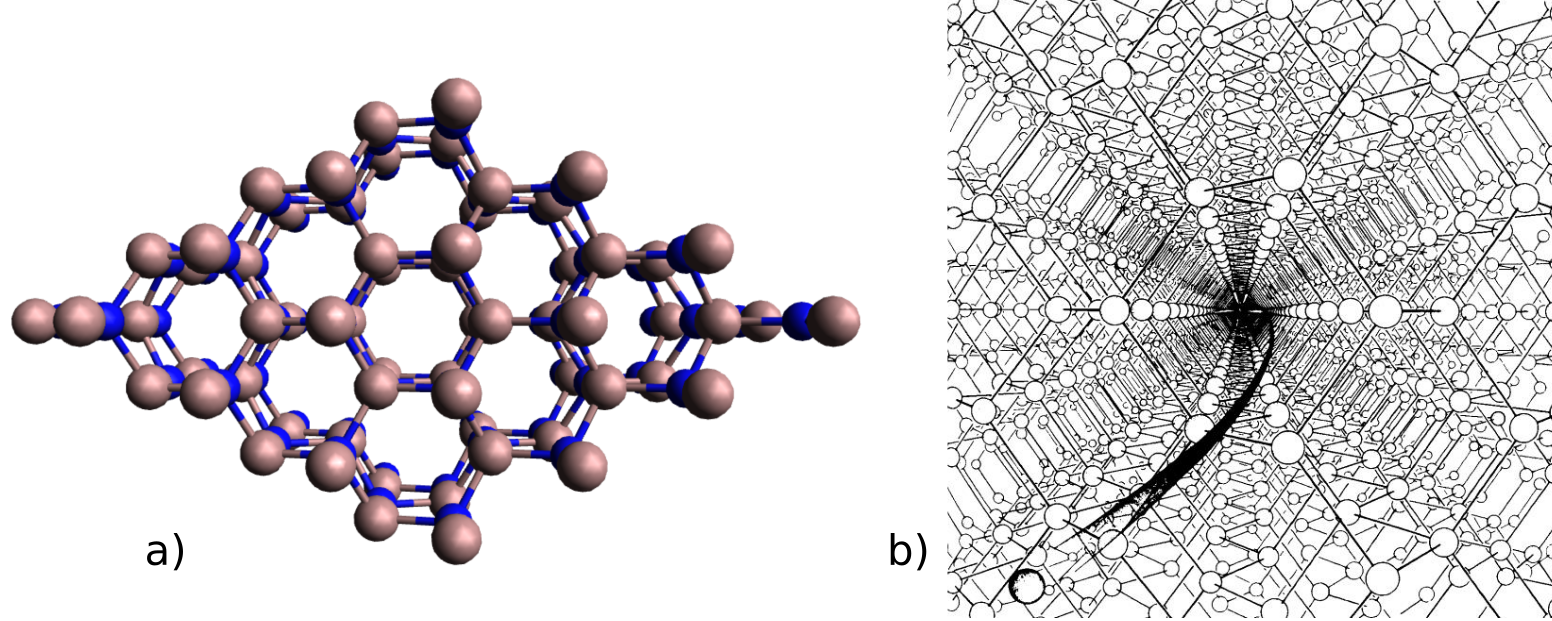
\includegraphics[width=1\linewidth]{Figures/channel2.png}
\caption[``Channels'']{ a) Open ``channels'' between rows of atoms along the main direction \hkl[001] in GaN -- \emph{not} responsible for what is sometimes called electron ``channelling''. b) Artist's impression of channelling of heavy charged particles, from~\cite{Brandt68} .}
\label{Fig:channels}
\end{figure}
%---------


These two SEM techniques carry the word \textit{channelling} for historical reasons. In early 1960s, before electrons became widely used in high resolution microscopy, ions were used in much the same way as electrons are in the scanning electron microscope. It was observed that the scattered secondary electron intensity depended on the ions' incident direction~\cite{Davies83}. This was in sharp contradiction with the 
theory of scattering at the time which assumed the distribution of atoms in samples can be approximated to a dense gas. It became apparent that an incident ion beam aligned along any of the major axes of the crystal would yield longer penetration depths, would loose energy slower and would generate fewer secondary electrons close to the surface~\cite{Piercy63}. This was initially explained as simple geometrical transparency, \ie columns of empty space along major axes as shown in Fig.~\ref{Fig:channels} a), such that the ions would simply suffer less scattering on their path as shown in the beautiful artist render in Fig.~\ref{Fig:channels} b) hence the name \textit{channelling}.


Based on these observations, Linhard~\cite{Lindhard65} developed a classical mechanics explanation for incident particles with small and incoherent wavelengths such that effects such as interference patterns can be ignored. He defined the condition for the validity of this classical treatment through the requirement that the number of bound states in the atom string potential to be large compared to unity ($\nu_s\gg1$). The full explanation of channelling is somewhat more involved then a simple geometrical transparency. The heavy particles, when incident at a direction close to a major crystallographic direction, behave as if focused by the total sum potential of the strings of atoms. Correlated deflection by the atoms in the strings protect the incident beam from penetrating close to the core of the atoms and suffer scattering. The resulting effect is that, in these special conditions, the incident particles can travel deeper in the sample and lose less energy, channelling, protected as they are by the potential of the string of atoms. Linhard then went on to establish an  upper limit for stable channelling for the incidence angle relative to a major direction he called the \textit{critical channelling angle}:

\begin{equation}
\theta_{chan} \leq \sqrt{\frac{2 Z e^2}{E d}} 
\end{equation} 
where $Z$ is the atomic number and $E$ is the energy of the incident particle, $e$ is the usual elementary charge and $d$ is the distance between atoms in the string.

Not only strings of atoms but also lattice planes can channel a beam of incident charged particles. In \textit{Notes on Channeling}, Andersen~\cite{Andersen14} explains the qualitative image of planar channelling analogous to the string of atoms channelling. The planar potential can be thought of as a superposition of string potentials, allowing the incident beam particles to sneak in between two strings and still be protected by the deflection of correlated atom scattering. The dark spot in the centre of the angular flux distribution in  Fig.~\ref{Fig:icp} a) is due to lower scattering rates along the direction parallel to the \hkl[001] axis, or string channelling. The dark lines are the result of planar channelling in the family of planes \hkl{100} and \hkl{110}.    


%---------
\begin{figure}[ht]
    \centering
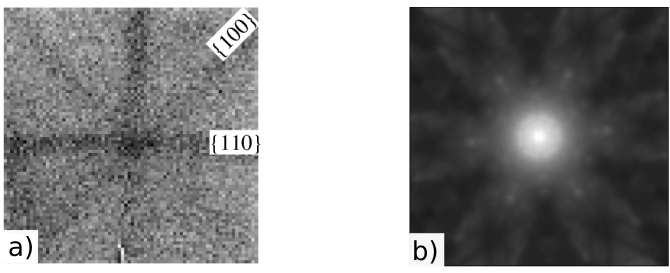
\includegraphics[width=0.66\linewidth]{Figures/icp-ecp.png}
\caption[Ion channelling.]{ a) Flux distribution of heavy ions scattered from a transmitted beam through \hkl[001] Si crystal, from~\cite{Assmann99}. b) Simulated ECP pattern of \hkl[001] GaN using EMsoft~\cite{EMsoft}. While the observed features are similar, a)~is an effect of channelling and b)~of diffraction.}
\label{Fig:icp}
\end{figure}
%---------





It was soon observed that the channelling extends to other charged particles like high energy protons~\cite{Dearnaley68} or alpha particles. For electrons and positrons, the first indications of crystal lattice influence on the scattering directions was given by observing emission yields from samples doped with $\beta^+$ emitters~\cite{Uggerhoj68}. It appeared that the scattered yield increased when electrons were travelling along a lattice direction. These observations were later confirmed by Rutherford scattering experiments of fast electrons incident on a sample~\cite{Uggerhoj69}. It was only natural to make the parallel with ion scattering experiments and the so called phenomenon of \textit{channelling}.  

Mysterious is the fact that Coates had already published, two years previously, his observation of Kikuchi like patterns in the SEM~\cite{Coates67} -- bright lines of increased electron backscatter intensity associated with lattice planes, yet the connection between the two phenomena was not made. By the time Joy wrote his significant contribution to the description and understanding of directional dependence of scattering in the SEM~\cite{Joy82}, the name of channelling had already gained traction and the phenomenon was known as an electron channelling pattern. When comparing the angular distribution of scattered ions (Fig.~\ref{Fig:icp} a) ) with that of electrons (Fig.~\ref{Fig:icp} b) ), the similarities are indeed indisputable. The contrasting lines in both cases are due to the lattice planes. In the first case the lines are dark indicating a lower scattering rate of ions when close to lattice directions and planes. However, in the electron case, the lines are bright, indicating an increase in scattering when electrons are close to the planes or directions. 

For a polycrystalline sample, the contrast in intensity from one grain to the other seems similar when using ions~\cite{Franklin88} and electrons. Since for ions it was attributed to channelling it only made sense to blame channelling for a change in electron yield (contrast) for different orientated grains (Electron Channelling Contrast Imaging). When we say electron channelling we only mean channelling in the sense of a stable trajectory close to atoms and planes. Nevertheless, the underlying physics is different. 

\begin{table}[ht]
\caption[Critical channelling angle]{Critical channelling angle $\theta_{chan}$ and Bragg angle $\theta_B$ for heavy ions and electrons travelling along \hkl(001) planes in a GaN sample. The number of bound states for strings $\nu_s$ and planes $\nu_s$ indicate the validity of the classical description of channelling. }
\label{table:channelling}
\centering
\begin{tabular}{ l l c c c c }
\toprule
\tabhead{Particle} & \tabhead{Energy [\si{\mega \electronvolt}]} & \tabhead{$\nu_s$ (classical?)} & \tabhead{$\nu_p$ (classical?)} & \tabhead{$\theta^{chan}$ [\si{\degree}]} & \tabhead{$\theta_B$ [\si{\degree}]} \\
\midrule
  C ion     &  1     & $>10$ (yes)            & $>10$ (yes) & $\leq 1.2 $           & $\leq 10^{-4}$\\
  electron  &  1     & $\approx 4$ (uncertain)& $< 1$ (no)  & $\leq$ \textit{0.1}   & $< 0.1$ \\
  electron  &  0.02  & $< 1$ (no)             & $< 1$ (no)  & $\leq$ \textit{0.9}   & 0.5\\
\bottomrule
\end{tabular}
\end{table}

For MeV ions, with short wavelengths, the interference effects can be safely ignored since mean free path for inelastic scattering is as short as a few lattice spacings. Meanwhile, for fast electrons we cannot ignore that at Bragg angles their scatter amplitude will interfere constructively, which is what gives the strong, sharp peak in the scattered yield. The legitimacy of a classical description, such as channelling, for explaining these peaks is, nevertheless, doubtful. 




In Table~\ref{table:channelling} I calculated the number of bound states, for both strings of atoms ($\nu_s$) and planes ($\nu_p$), for electrons at \SI{1}{\mega \electronvolt} and \SI{20}{\kilo \electronvolt} scattered along \hkl(001) planes in GaN. For electrons, the number of bound states in the string potential can be reduced from~\cite{Lindhard65} to:
\begin{equation*}
\nu_s \approx \frac{1}{\sqrt{1-\frac{v^2}{c^2}}}\,\, Z^{1/3} \,\, \frac{4a_0}{d}
\end{equation*}
and the number of bound states in a planar potential to:
\begin{equation*}
\nu_p \approx \frac{0.4}{(1-\frac{v^2}{c^2})^{1/4}} 
\end{equation*}
where $Z$ is the atomic number of the target material, $a_0$ is the Bohr radius, $d$ is the distance between atoms in a string and $v$ is the speed of the incident particle~\cite{Uggerhoj69}.  

Diffraction and channelling are two separate but competing phenomena~\cite{Chadderton70}. They are defined by the Bragg and channelling angle, respectively, and looking at the range of these parameters we can decide which of these events dominates. For electrons with energies below \SI{1}{\mega \electronvolt} the classical description is not appropriate, and the critical channelling angle is meaningless, which is why I wrote it in italics. But, for very high energy electrons, with energies above \SI{1}{\mega \electronvolt}, channelling can become a relevant phenomena and will compete with the Bragg angle. We can see the situation is reversed for heavy ions, which are highly localised with numerous bound states, both in the string potential and the planar potential. However, the Bragg angle is vanishingly small for these heavy particles and therefore diffraction effects can be ignored. 

For SEM electron energies we are comfortable in the non-channelling range. Nevertheless, we will continue to use Holy-Roman-Empire-names of Electron Channelling Pattern and Electron Channelling Contrast Imaging and understand that the word channelling in these cases is different from the effect of ions channelling, referring instead to stable trajectories close to atomic nuclei for the electron Bloch waves. 



Winkelmann and Vos~\cite{Winkelmann13} describe in detail the mechanism of \textit{channelling in} means for ECPs and \textit{channelling out} for EBSD.




%%%%%%%% %%%%%%%%
 \section{Electron channelling contrast model}

Dislocation contrast is a term coined for transmission electron microscopy. Defect characterisation in TEM is relatively well established. Both qualitative models such as the kinematical theory~\cite{Hirsch60}, and more quantitative models in the form of the dynamical theory~\cite{Howie61,Clarke71,Spencer72} have been developed and successfully applied to predict dislocation contrast.

%TEM thin samples 
We have mentioned before that TEM samples must be prepared to be very thin. This is usually required in order to maximise the number of electrons that will escape from the bottom side of the sample. It is these very thin samples that minimise the interaction volume of the electrons that make the approximations in the original version of the dynamical theory pertinent. 

%SEM thick sample probably should account for absorption
For thicker samples than the ones used for TEM, inelastic scattering of electrons becomes impossible to ignore. When electron paths become long enough, a significant number of them are removed or ``absorbed'' from the diffracted beam through inelastic scattering. This loss becomes important when we take into account the dynamical pendell{\"o}sung of intensities between the the direct and diffracted beams. We will, therefore, always take into account absorption through the optical lattice potential discussed on page~\pageref{sec:absorbtion}.


Otherwise, we will follow the path paved by TEM contrast simulations. This involves, simply correcting the deviation from the Bragg condition for the existence of a dislocation nearby. This correction, which we will call $\beta$, is, to a first approximation the directional derivative of the dislocation displacement field along the diffraction vector \textbf{g}. We will see in Section~\ref{sec:beta} on page~\pageref{sec:beta} that we will add a second order correction.  

We then start again from the general Darwin-Howie-Whelan equation (Eq.~\ref{eq: multiDHW}), but this time we add the dislocation  correction:
\begin{equation}
\label{eq: multiDHWTD}
     \frac{d \psi_\mathbf{g}}{dz_{beam}} - 2 \pi  (\vb{s}_g+ \beta) \psi_{\vb{g}} = i \pi \sum_{\vb{g}'} \left( \frac{ e^{i \theta_{\textbf{g}- \textbf{g'}}}}{\xi_{\vb{g}-\vb{g}'}} +i\frac{ e^{i \theta'_{\textbf{g}- \textbf{g'}}}}{\xi'_{\vb{g}-\vb{g}'}}\right) \psi_{\vb{g}'}.
\end{equation}


These equations, now become too complicated for an analytical solution and, as we will see in Section~\ref{sec:numerical} on page~\pageref{sec:numerical},  we need to use a computer to solve numerically. 

Let us, in the following pages, talk about how to calculate the corrections needed for the DHW equations from the displacement field of dislocations. 


 %%%%%%%%%%%%%
 \section{TDs displacement field for ECCI}
 \label{sec:strain}


We are now tasked to calculate the displacement field introduced by a dislocation in a perfect crystal and for this we turn to elasticity theory. 

Even one dislocation will disturb every single one of the $\approx 10^{11}$ atoms in one micrometer cube of the sample in a non trivial manner, the effects of this distortion can then affect the phase of the diffracting electrons and can be resolved in the SEM. In order to simulate this complex multi body problem it is not unwise to turn to a model that would strip down all unessential details to the bare physical properties that drive these interactions.

This branch of continuum mechanics developed specifically for the description of dislocations brings many elegant simplifications to the treatment of dislocations, but also some limitations. In the following subsections we are to direct our attention towards the derivation of strain fields produced by threading dislocations running normal to the surface of a sample using this mathematical formulation.

\subsection{Elasticity theory}
 As part of continuum mechanics, elasticity theory ignores the fact that matter is made out of discrete particles and instead approximates it to be continuous and uniform even at the microscopic level. This conveniently enables us to ignore the very complicated interaction between the many atoms as well as any discontinuing properties at the microscopic level (including the actual dislocations!) simplifying the treatment a great deal. Instead, it entertains the more intuitive idea that matter fills the entire region of space it occupies in a continuous and homogeneous manner and that this holds true for any infinitesimal region of space. While this is not a rigorous description at the microscopic scale, for the micrometer level study of structural effects of dislocations, these crude assumptions will hold fully.

In this model all the specific physical properties of the continuum are exactly the same for
any infinitesimal selected region. This facilitates the substitution of what would otherwise be discontinuous quantities with single valued, smooth fields representing the average value over that infinitesimal region of space of the property we would want to study. 

In continuum mechanics we are concerned with the stress field applied to a material and the strain response of said material. Notice the word field in the previous statement. Many material properties are not simple scalars. In this case, both the strain and stress are tensors of rank 3 as shown in Fig.~\ref{fig:stress}. Not all of the $3\times 3$ matrix components are necessarily unique. In fact, it turns out that these entities are intrinsically symmetric\footnote{Onsager’s Principle of Microscopic Reversibility~\cite{Onsager} can be used to show that principal transport properties are symmetrical tensors.} for a system at equilibrium, resulting therefore in only 6 unique components.  

%-------
\begin{figure}[ht]
    \centering
    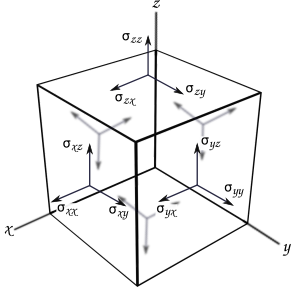
\includegraphics[width=0.42\linewidth]{Figures/cubefin.png}
    \caption{Stress distribution on an infinitesimal volume.}
    \label{fig:stress}
\end{figure}
%---------

Within the framework of continuum mechanics we also make the assumptions of \textit{linearity} and \textit{perfect elasticity}. The final approximation we will introduce is that of \textit{elastic isotropy}. We provide below the implications of these assumptions:
\begin{enumerate}
\item If a body returns to its original form completely after any deformation force is applied, we say that object possesses the property of \textit{perfect elasticity}. Mathematically this is achieved by keeping the forces that produce the deformation below the plasticity region of the structural material of interest, or in other words very small (small enough).

If we define $\sigma_{ij}$ as the $i^{th}$ component of the stress (force per unit area) on a plane whose normal is in the $x_{j}$ direction as shown in Figure~\ref{fig:stress}, and then consider that when acted upon by stress a body deforms such that the displacement at point \textbf{r} is \textbf{u} with component $u_{i}$ we can define strain as:
\begin{equation}
\label{eq:epsilon}
\epsilon_{ij}=\dfrac{1}{2}\left(\dfrac{\partial u_i}{\partial x_j} + \dfrac{\partial u_j}{\partial x_i}\right)
\end{equation}

\item In the equation above we have assumed the distortions are small enough that we can ignore all but first terms in the expansions of individual displacement components. This is also known as \textit{linearity} and also produces a linear relation between stresses and deformations (Hooke's law):
\begin{equation}
\label{eq:sigma}
\sigma_{ij}=c_{ijkl}\epsilon_{kl}
\end{equation}
where the coefficients $c_{ijkl}$ form a rank 4 tensor and are the elastic constants. For the most general case form a $6\times6$ matrix relating the six unique elements of $\sigma_{ij}$ to the six elements of $\epsilon_{kl}$. 

\item The final assumption we make here is to state that our material can be reduced to \textit{elastic isotropy} without impairing greatly the accuracy of the results. This is the property of a material whose elastic properties are independent on the orientation we study it in. This, in general, is not the case for none but a handful of cubic structures. For the wurtzite structure, Neumann's rule predicts all the symmetries of its point group. Additionally, since wurtzite is not that far crystallographically from zinc blende, it can be shown~\cite{Martin72} that one can reduce the wurtzite elastic constants to an effective cubic zinc blende tensor. This reduces the number of independent variables to three and we can rewrite Eq.~\ref{eq:sigma} as:

\begin{equation}
\begin{bmatrix}
\sigma_{11}\\
\sigma_{22}\\
\sigma_{33}\\
\sigma_{23}\\
\sigma_{13}\\
\sigma_{12}
\end{bmatrix}
=
\begin{bmatrix}
2\mu+\lambda  &  \lambda       &  \lambda       &  0 & 0 & 0\\
\lambda       &  2\mu+\lambda  &  \lambda       &  0 & 0 & 0\\
\lambda       &       \lambda  &  2\mu+\lambda  &  0 & 0 & 0\\
 0            &       0        &  0             &\mu & 0 & 0\\
 0            &       0        &  0             &0   &\mu& 0\\
 0            &       0        &  0             &0   & 0 & \mu
\end{bmatrix}
%
\begin{bmatrix}
\epsilon_{11}\\
\epsilon_{22}\\
\epsilon_{33}\\
2\epsilon_{23}\\
2\epsilon_{13}\\
2\epsilon_{12}
\end{bmatrix}
\end{equation}
with $\mu$ known as the shear modulus and $\lambda$ the Lam\'{e} constant. We can introduce another useful constant: the Poisson ratio, $\nu$:
\begin{equation*}
 \nu = \frac{\mu}{2(\mu + \lambda )}   
\end{equation*}

\end{enumerate}
However, no crystal structure is truly isotropic with the wurtzite crystal system showing an anistropy factor of 0.86 (compared to 1.0 for an isotropic system). Nevertheless, physics is all about approximating a complex system to a simple system and then adding corrections. This is exactly what the \textit{Voigt} formula~\cite{Hirthbook} achieves. In Table~\ref{Table:voigt} I give the elastic parameters for GaN if we are to approximate it to be isotropic. 

\begin{table}[ht]
    \centering
    \begin{tabular}{l c c}
    \toprule
        \tabhead{Elastic constant}    & \tabhead{Symbol} & \tabhead{Voigt approximation}  \\
    \midrule    
        Shear modulus    & $\mu$         & \SI{121}{\giga \pascal}  \\
        Lam\'{e} constant & $\lambda$    & \SI{129}{\giga \pascal}  \\
        Poisson ratio    & $\nu$         &  0.26\\
    \bottomrule     
    \end{tabular}
    \caption[Wurtzite GaN Voigt elastic constants.]{Voigt approximation of elastic constants for isotropic wurtzite GaN.}
    \label{Table:voigt}
\end{table}



 %%%%%%%%%%%%%%%
 \subsection{Semi-infinite screw dislocation}
A screw dislocation is a shear in the crystal with the edge of shear being the dislocation line itself. The amount of shear is quantified in terms of lattice parameters and is a vector along the dislocation line. This vector quantifying displacement is known as the \textit{Burgers vector}, $\textbf{b}$.  

Let us work out the displacement introduced by a screw dislocation in a perfect crystal. The screw dislocation, let's say aligned with  the \textit{z}-axis,  introduces displacement only along the dislocation line, as comprehensibly explained in \textit{Theory of dislocations}~\cite{Hirthbook}:
\begin{equation}
    u_z = \frac{b}{2\pi}\arctan{\frac{y}{x}}
\end{equation}
 From Eq.~\ref{eq:epsilon} we can conclude that the only strain components produced by this displacement must be $\epsilon_{xz}$ and $\epsilon_{yz}$. If we were now to consider a surface on which the dislocation is normal, both these strains will act on the surface and the surface itself will have an effect on the displacement field of the dislocation. 
 
\textit{Saint-Venant's principle}~\cite{StVincent} tells us that the forces exercised by a surface on an elastic body are equivalent to replacing the surface by an object impacting the same force as long as the object is far away. So far this is not particularly unsettling. The beautiful approach based on this concept is that we can talk of the effect of surface relaxation around a dislocation as being derivable, similarly to the electrostatics world, by adding an imaginary field that ensures the surface ``feels'' zero strain. 
 
 In our case, for a screw dislocation normal to a surface, it is the out of plane stress that must be relaxed. The relaxation displacements in Cartesian coordinates was calculated by Eshelby and Stroh~\cite{Eshelby51} to be simply:
\begin{align}
u^i_x =& \dfrac{b}{2\pi}\dfrac{y}{r-z}\\
u^i_y =& -\dfrac{b}{2\pi}\dfrac{x}{r-z}
\end{align}

In the end, the total displacement introduced by a TD normal to a surface is made up of the $real+imaginary$ displacement fields.  
In Appendix~\ref{Chap:strainMatrix}, Fig.~\ref{Fig:screwMatrix} I show the elastic strain tensor components as contour plots for a screw TD in GaN using Eq.~\ref{eq:epsilon} with the displacements shown here.



%%%%%%%%%%%%%%%%%%
\subsection{Semi-infinite edge dislocation}

An edge dislocation is the result of introducing an extra plane of atoms in a perfect crystal. The displacement field introduced is in plane and is given in Cartesian coordinates in the notation from \cite{Indenbom} as:
\begin{align}
    u_x =& \frac{ b }{2\pi} \left[\arctan{\frac{y}{x}} + \frac{xy}{2(1-\nu)(x^2+y^2)}\right]\\
     u_y =& -\frac{ b }{2\pi} \left[\frac{1-2\nu}{4(1-\nu)}ln(x^2+y^2) + \frac{xy}{4(1-\nu)(x^2+y^2)}\right]
\end{align}

The surface relaxation is more involved in this case, but Yoffee derived an elegant solution~\cite{Yoffe} for a dislocation interacting with a surface at a general angle:
\begin{align}
u^i_x ={} & \dfrac{\nu b}{4 \pi(1-\nu)} \left[\dfrac{2xyz}{r(r-z)^2}+(1-2\nu)\dfrac{xy}{(r-z)^2}\right] \\
u^i_y ={} & \dfrac{\nu b}{4 \pi(1-\nu)} [(1-2\nu)\log(r-z) - (3-2\nu)\dfrac{z}{r-z}   \notag \\
          &{} \qquad \qquad \qquad \qquad  \qquad  \qquad + (3-2\nu)\dfrac{y^2}{(r-z)^2} - \dfrac{2y^2}{r(r-z)}]     \\  
u^i_z ={} & \dfrac{\nu b y}{2\pi(1-\nu)} \left[\dfrac{1}{r} + (1-2\nu)\dfrac{1}{r-z}\right]
\end{align}

Such that the total displacement components are: $u^t_x = u_x + u^i_x$, $u^t_y = u_y + u^i_y$, $u^t_z =  u^i_z$. In Appendix~\ref{Chap:strainMatrix}, Fig.~\ref{Fig:edgeMatrix} I show the elastic strain tensor components as contours plots for an edge TD in GaN using Eq.~\ref{eq:epsilon}  with the displacements shown here.




%%%%%%%%%%
\section{Correction \texorpdfstring{$\beta$}{beta} to \texorpdfstring{$\mathbf{s}_g$}{sg} due to TD strain}
\label{sec:beta}
The image of a single crystal surface in high magnification mode should consist of a constant backscattered electron yield as the near parallel beam is scanned over a small area. Around a dislocation line the crystal structure is distorted, which in turn affects the diffraction of the electron beam. The shift in diffraction behaviour close to the dislocation is observed as a change in the number of backscattered electrons originating from the distorted crystal region and provides direct information about departures from the perfect crystal structure in the ECCI micrograph. Similarly to the contrast mechanism in TEM described by Hirsch~\etal~\cite{Hirsch60}, the lattice curvature directly affects the distance by which the diffracting reciprocal lattice points deviate from the Bragg condition and is quantified by the deviation parameter $\mathbf{s}_g$. The correction needed to account for the distortion introduced by a lattice defect is then the change in the direction of the incident electron beam, $\mathbf{r}_{inc}$, of the component of the displacement field, $\mathbf{u}$, which is parallel to the reciprocal vector, $\mathbf{g}$, defining the diffraction condition. Tunstall~\etal~\cite{Tunstall64} showed geometrically that there is a second, smaller correction term which accounts for the change in lattice parameters close to the dislocation:
\begin{equation}
\label{eq:tunstall}
    \mathbf{s}'_g = \mathbf{s}_g + \beta = \mathbf{s}_g + \mathbf{\hat{r}}_{inc} \cdot \nabla(\mathbf{u} \cdot \mathbf{g}) + \theta_B \mathbf{\hat{r}}_{g} \cdot \nabla(\mathbf{u} \cdot \mathbf{g} )
\end{equation}
where $\theta_B$ is taken to be the Bragg angle and $\mathbf{\hat{r}}_{g}=\mathbf{r}_g/ |\mathbf{r}_g|$  is the coordinate in the dislocation frame parallel to $\mathbf{g}$.

The new variable $\beta$ is the sum of all corrections to the deviation parameter due to the defect. If defined in an orthogonal coordinate system it can also be written as:
\begin{equation}
\label{eq:beta}
    \beta = \frac{\partial u_g}{\partial r_{inc}} + \theta_B\frac{\partial u_g}{\partial r_g}
\end{equation}
where $u_g$ is the displacement field in the direction of $\mathbf{g}$.

 If the displacement field is defined in a Cartesian reference frame in which $\mathbf{g}$ is parallel to one of the axes then the corrections terms above can be considered as strain-like components since they measure displacements field gradients. Due to the $\theta_B$ weighting factor, the second strain-like term introduced by Tunstall is negligible and can be ignored whenever the first term is non-zero as we will see later. It is these strain-like components that disturb the electron diffraction as compared to a perfect crystal and generate the dark-bright contrast features associated with dislocations in ECCI images.
 
%%%%%%%%%%     
\subsection{The failure of the invisibility criterion for ECCI}

We mentioned a few times that transmission electron microscopy has established itself as the default technique for the study of lattice deformations. It is especially reliable as a dislocation characterisation method as it can identify unambiguously the $\mathbf{c}$ and $\mathbf{a}$ components of a dislocation line running parallel to the imaged surface. This is achieved through the application of certain relationships between the diffraction vector $\mathbf{g}$, Burgers vector $\mathbf{b}$ and the direction of the dislocation line $\mathbf{u}_l$ ($\mathbf{g} \cdot \mathbf{b} = 0$ and $\mathbf{g} \cdot \mathbf{b} \times \mathbf{u}_l = 0$), known as the invisibility criteria, for which no contrast associated with $\mathbf{c}$ or $\mathbf{a}$ components, respectively, can be observed. This method has been applied broadly in the study and characterisation of dislocations in cross sectional GaN samples, \eg ~\cite{Hino00}.


Let us briefly discuss why, unlike the case for cross-section TEM, the invisibility criterion is not appropriate for dislocation identification in the forescatter geometry of ECCI especially in the absence of high resolution electron channelling patterns (ECPs).

The displacement in an infinite lattice due to a dislocation line of type $\mathbf{a}$ or $\mathbf{c}$ can be derived from elasticity theory in the linear regime (see for example Ref.~\cite{Read53}). If the dislocation line interacts in any way with the free surface of the layer, the non-zero stresses at the interface have to be relaxed in order to obtain the full strain picture of the dislocation line. This relaxation in turn introduces extra displacements such that the total displacement at any point in the lattice is a sum of the ``infinite-lattice'' displacement and that due to the surface relaxation. Yoffe~\cite{Yoffe} has calculated these surface relaxations due to general dislocations intersecting the surface at an arbitrary angle.

The importance of surface relaxation in the simulation of the electron channelling contrast micrograph has already been discussed by Wilkinson~\etal~\cite{Wilkinson95} for dislocations running parallel to a nearby surface. Even for the diffraction conditions where the infinite-lattice model gives no ECCI strain-like components, the non vanishing surface strain terms ensure that the net contrast will never be truly zero. This effect will only increase for dislocation lines which penetrate the surface where the non-vanishing surface terms become even more significant. Even in the case where the Burgers vector is perpendicular to the $\mathbf{g}$ direction, the ECCI sampled strain will be smaller but still not zero.

This reduction in dislocation contrast at the invisibility criteria had been already used in literature~\cite{Morin79, Crimp01} to show that, at least phenomenologically, the same principle can be applied to ECCI. In practice care is advised when using this approach for the characterisation of dislocations. Unlike TEM which allows reasonable dislocation contrast to be acquired for a significant range of deviations from the Bragg condition, the contrast in ECC images is optimised at the exact Bragg condition, $\mathbf{s}_g = 0$, and can change drastically on small variation from that condition. This can determine whether a dislocation is visible or not, even for diffraction conditions where we would expect to see good contrast (see also the discussion in Ref.~\cite{Crimp06}).


%%%%%%%%     
\subsection{ECCI strain profile for the forward scattering geometry}
\label{sec:tilteffect}

\begin{figure}[ht]
    \centering
    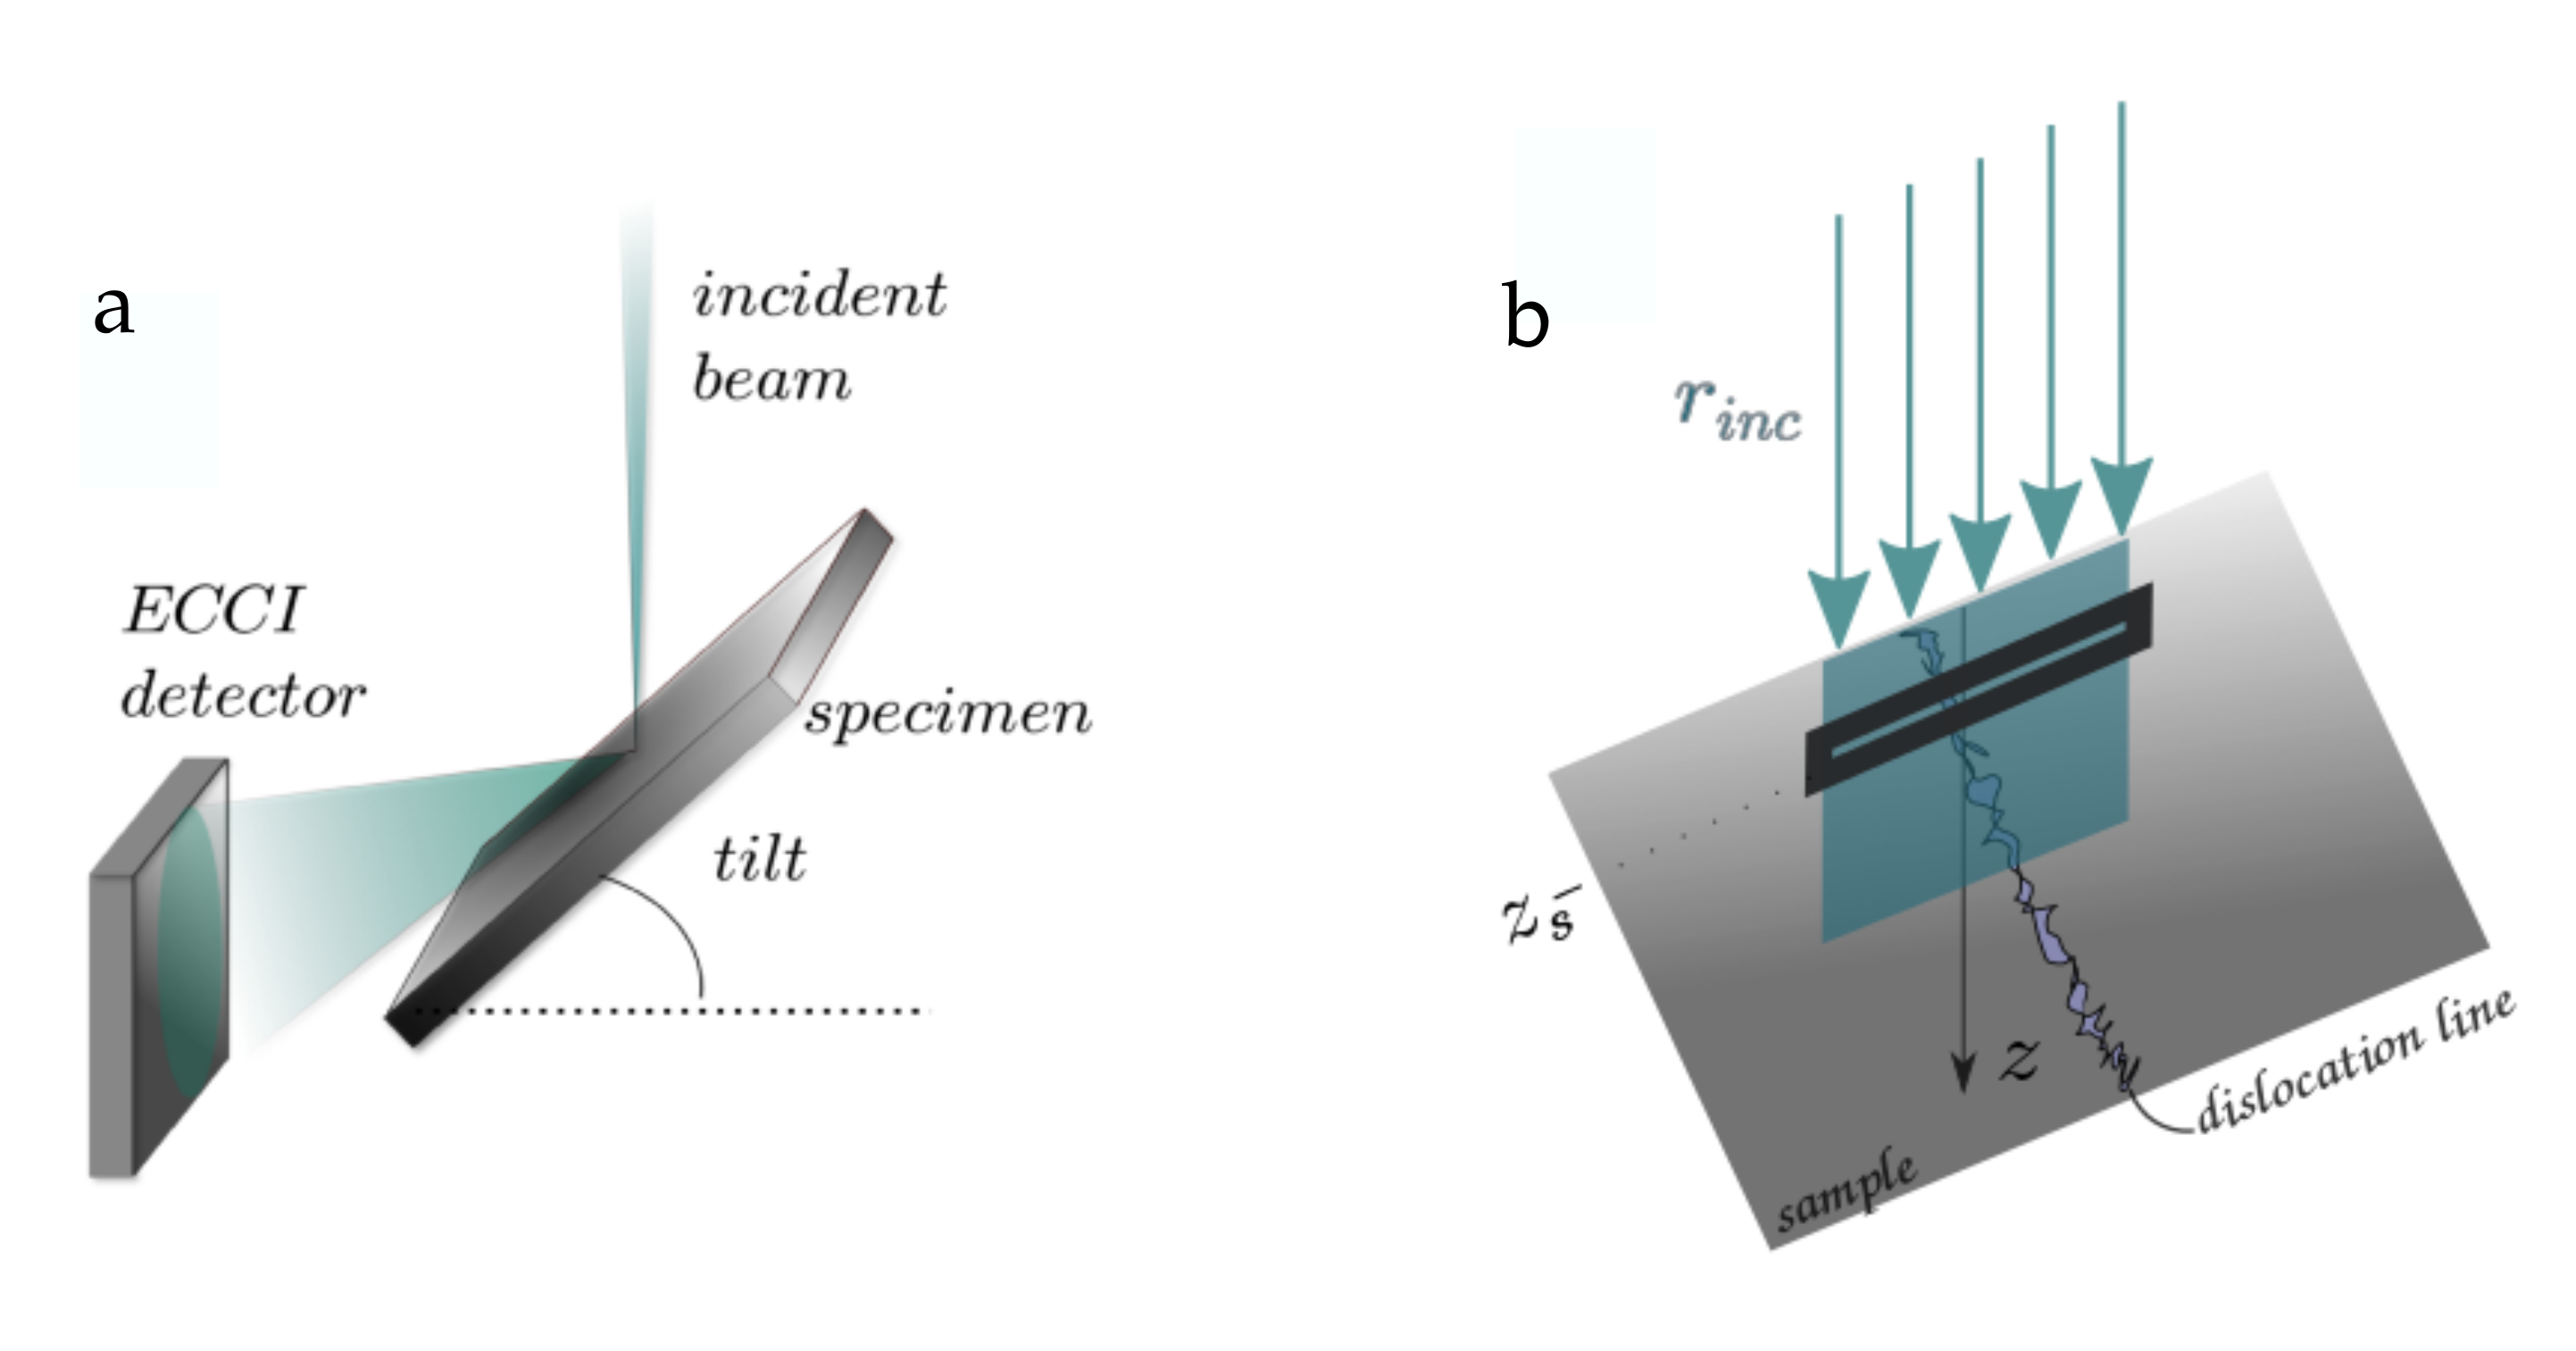
\includegraphics[width=0.8\linewidth]{Figures/forward_geom.png}
    \caption[Forward-scattering geometry.]{a) Schematic of forward-scattering geometry in the SEM. b) The geometry of the incident beam with respect to a tilted sample. The rectangular box shows the plane $z_s$ which is considered in Fig.~\ref{fig:tilting_eff}.  }
    \label{fig:tilt}
\end{figure}

From Eq.~\ref{eq:beta} we can see that the strain profile imaged by ECCI, $\beta$,  of the \textbf{a} character of a TD normal to the surface is sensitive to variations in the angle of incidence of the electron beam, $r_{inc}$. This is indeed the case for the forward-scattering SEM geometry; I show what I mean by this schematically in Fig.~\ref{fig:tilt}. This effect is especially strong for edge TDs because they introduce elastic displacement mostly in the plane normal to the dislocation line and present almost no variation along a normally incident beam. Shown schematically in Fig.~\ref{fig:tilting}, the strain-like component only contains surface terms and anisotropy effects. Titling the sample (or the beam) translates to rotating the coordinate system in which the ECCI strain is defined, which means the tensor element in the new system will have to contain components from the plane normal to the dislocation line.

\begin{figure}[ht]
    \centering
    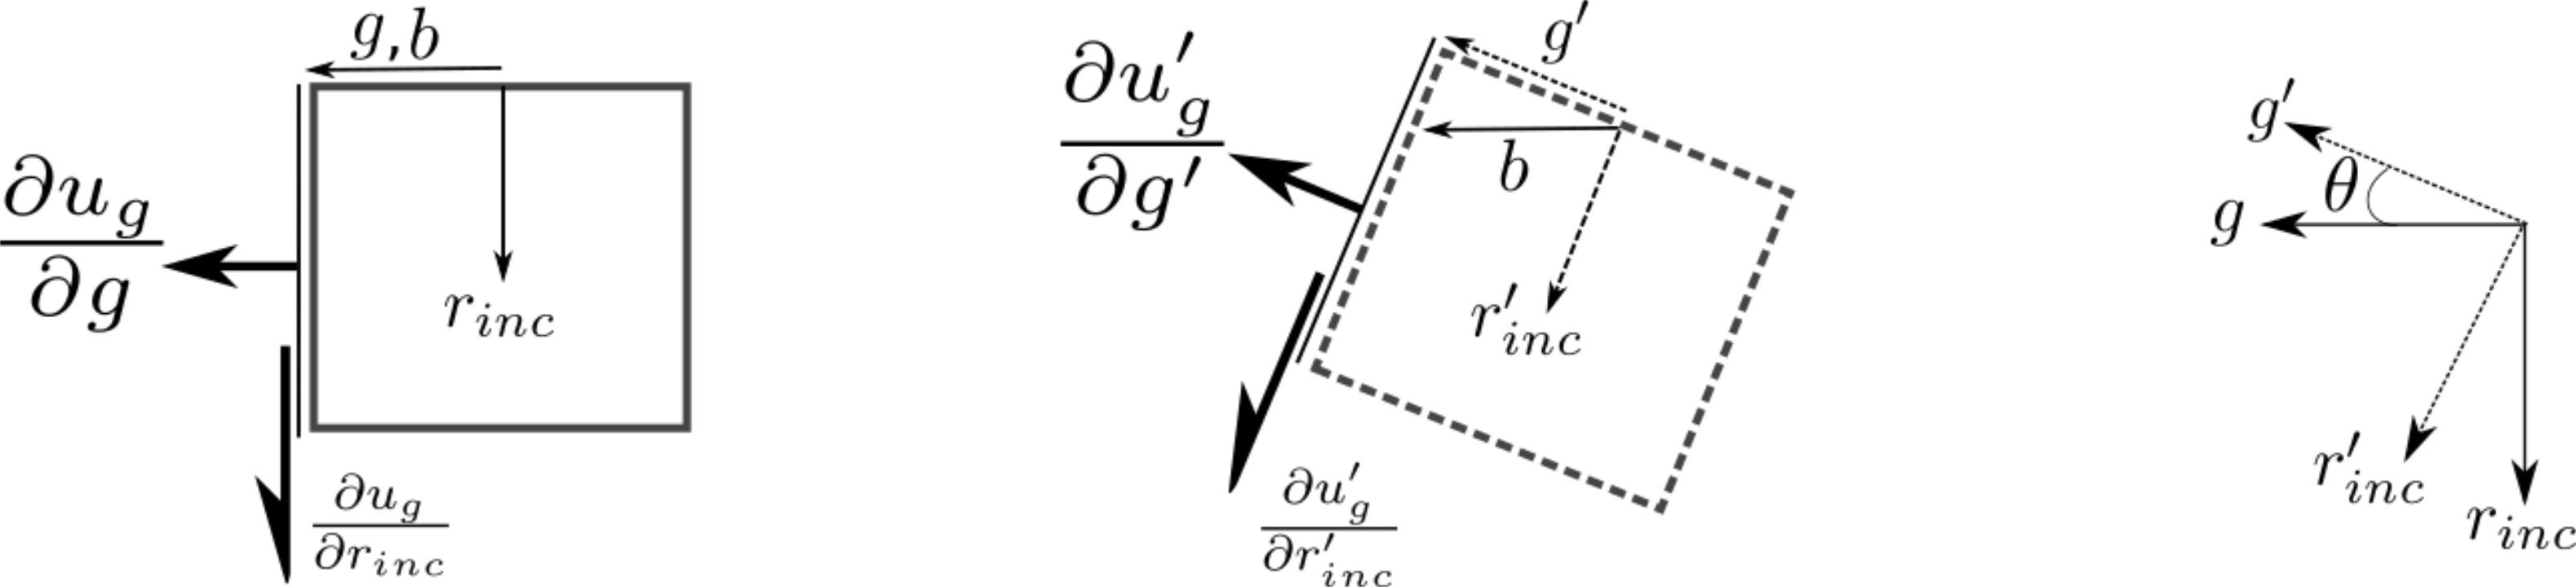
\includegraphics[width=0.9\linewidth]{Figures/tilting.png}
    \caption[Rotation transformation of sample tilting.]{2D diagram of rotation transformation in ECCI strain tensor. A $\theta$ clockwise rotation of the sample is equivalent to the same rotation of the coordinate system in which the strain components are defined. }
    \label{fig:tilting}
\end{figure}


The diagram in Fig.~\ref{fig:tilting_eff} illustrates this in two dimensions in the case when \textbf{b} is parallel to\textbf{ g}. For a clockwise rotation of the sample around a direction normal to both the dislocation line and its \textbf{b}, the first term of in the new coordinate system will be:
\begin{equation*}
    \frac{\partial u'_g}{\partial r'_{inc}} = \cos^2{\theta}  \frac{\partial u_g}{\partial r_{g}} + \sin{\theta} \cos{\theta}  \frac{\partial u_g}{\partial r_{inc}}
\end{equation*}
where the terms measuring the variation of the displacement field in the beam direction are ignored as they are
very small. The first part in the equation above is the variation of the displacement field along \textbf{b} (or \textbf{g} in this case) and for reasons discussed above will be the dominant term in this strain expression. More about transformation of coordinates will be addressed in next subsection.



It is to be expected, then, that tilting the sample will improve the observed contrast of edge dislocations significantly. Fig.~\ref{fig:tilting_eff}  a) to c) show how a small tilt can significantly change not only the intensity of the sampled strain but also the orientation of its high-low profile. This second effect has to do with the fact that our definition of $\beta$ (Eq.~\ref{eq:beta}) contains two strain-like components. Since the variation of displacement field along the line direction  (the first term of Eq.~\ref{eq:beta}) for the \textbf{a} character of a threading dislocation is negligibly small, what we observe in Fig.~\ref{fig:tilting_eff} a) is purely the second strain-like component introduced by Tunstall. This strain profile closely resembles TEM bright field intensity maps for an edge dislocation normal to the foil surface computed by Tunstall \etal~\cite{Tunstall64}  with the high-low ``butterfly'' lobes oriented on each side of the Burgers vector.

\begin{figure}
    \centering
    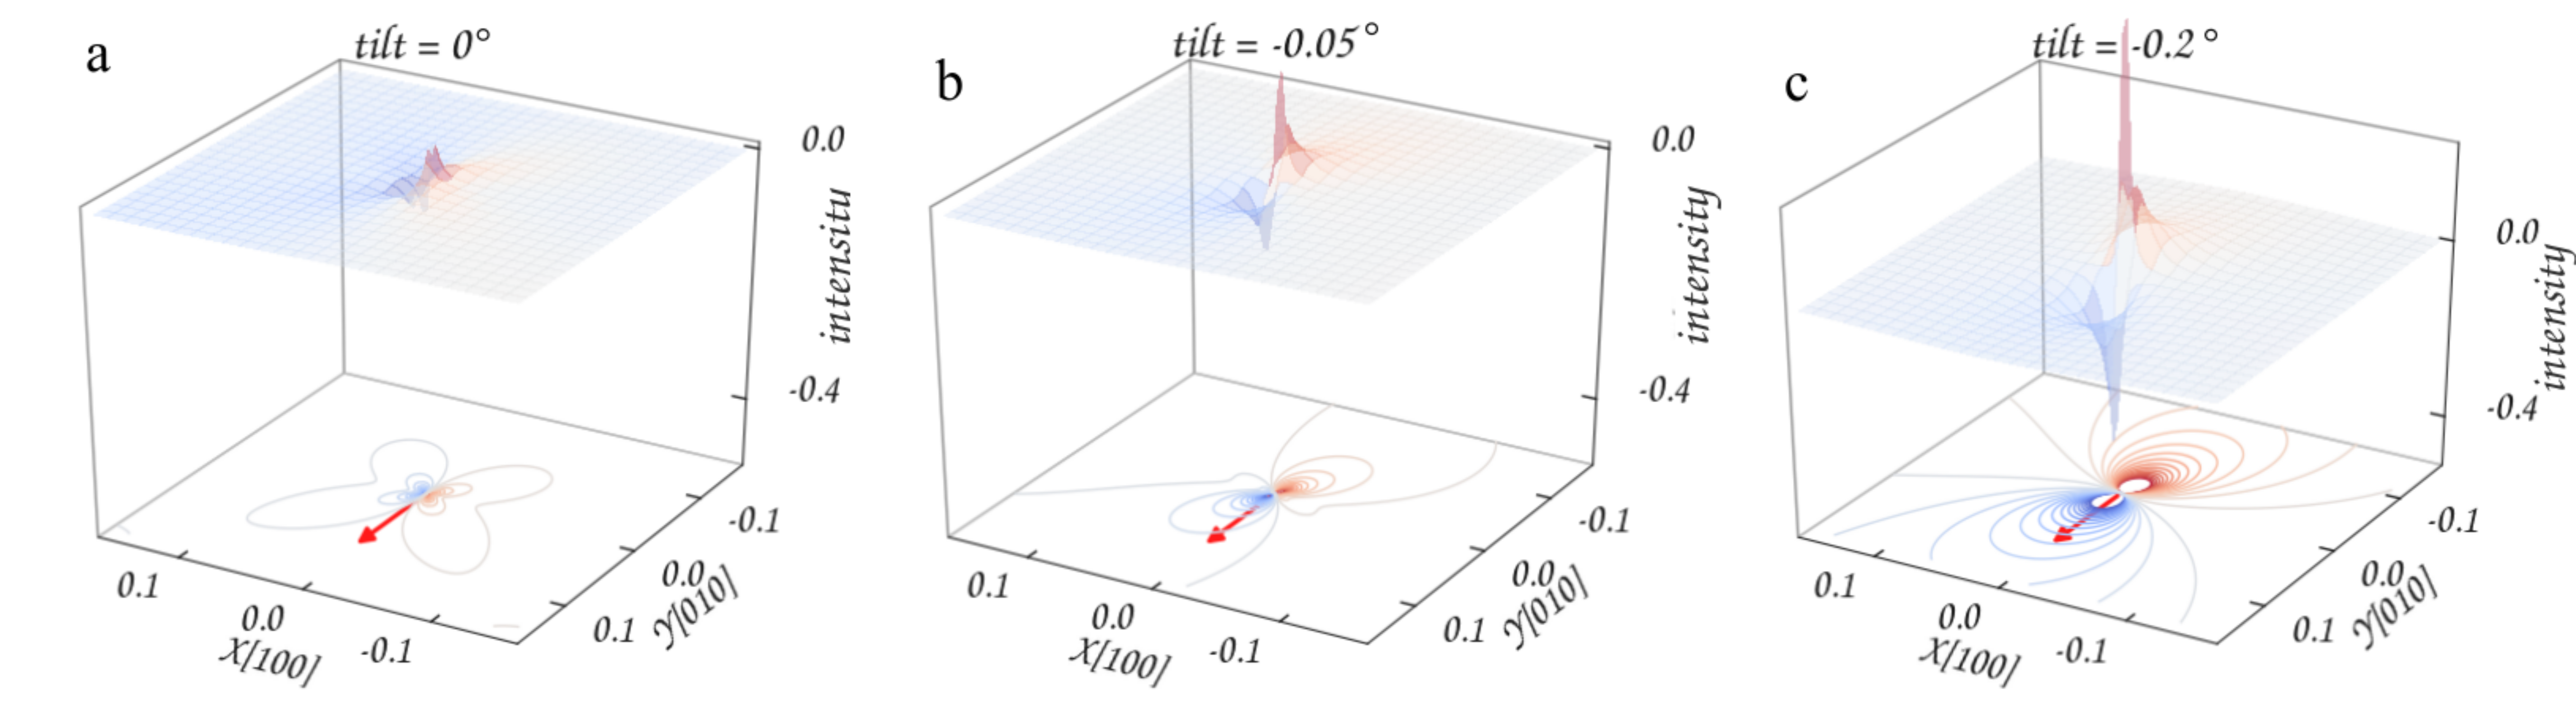
\includegraphics[width=1.1\linewidth]{Figures/tilting_effect.png}
    \caption[Planar edge TD $\beta$ strain profile. ]{The $\beta$ strain profile due to an edge TD in a cubic material shown in a plane $z_s$ parallel to the surface for three electron beam incidence angles close to zero a) \SI{0}{\degree}, b) \SI{-0.05}{\degree} and c) \SI{-0.2}{\degree}. The red arrows show both the Burgers vector direction and the projection of \textbf{g}.}
    \label{fig:tilting_eff}
\end{figure}

However, Tunstall’s component is orders of magnitudes less significant than the first term of $\beta$, $\frac{\partial u_g}{\partial r_{g}}$. This means that when the foil is tilted, Tunstall’s strain profile will be replaced by the profile of the first term. It is remarkable that, in the case when the diffraction vector is aligned parallel with the Burgers vector, any amount of sample tilt will change the direction of the minimum-maximum strain direction from being perpendicular to \textbf{b} to being parallel.
When the full three dimensional displacement field is considered it becomes apparent that the variation of the field
along the extra plane of atoms introduced by the edge dislocation dominates all other factors and this function has its
maxima and minima along the Burgers vector. This contrast alignment was observed experimentally and reproduced
by simulations for threading dislocations inclined to the surface by Picard \etal~\cite{Picard}.

The images in Fig.~\ref{fig:tilting_eff} also highlight the ability of forescatter geometry ECCI to access the TD strain profile for cases where plan view imaging might produce low signal to noise features. In general, the higher the tilt, the better the expected contrast of edge TDs will be.




%%%%%%%%%%%
\subsection{General coordinate transformation}
\label{sec:coordinates}
Eq.~\ref{eq:tunstall} contains mathematical objects specified in various reference frames and are therefore described using different basis sets. The \textbf{g} vectors are described in the reciprocal crystal frame, the displacement field is defined in the dislocation frame and the incident beam and sample orientation are usually given in lab coordinates. The first component of $\beta$ in Eq.~\ref{eq:tunstall} for instance, can be written to show explicitly the relationship between reference frames, following the notation used by De Graef~\cite{MarcTEM03} as:
\begin{equation}
    \frac{d \mathbf{u}(\mathbf{r}) \cdot \mathbf{g}}{d r_{inc}} = (r_{inc})^d_i \, \frac{\partial u^d_j}{\partial x_i} \mathcal{T}^{ds}_{js} \, B_{lm} g_m
\end{equation}
where Einstein summation convention is used for repeating subscript indices. The superscripts indicate the reference frame in which the expression of the vector is known. $B$ is the reciprocal structure matrix for the unit cell of the material.  $\mathcal{T}^{ds}_{js}$ is the coordinate transformation matrix which can be applied to a vector described in the dislocation frame ($d$) in order to be translated in the sample frame ($s$).

Fig.~\ref{fig:sampleframe} shows the relationship between the lab frame, the sample frame and the dislocation frame as well as the rotations required to orient one with respect to the others. For instance, the sample is rotated clockwise with the angle $\alpha_{rot}$ about the $x$ axis direction with respect to the lab frame.

\begin{figure}[ht]
    \centering
    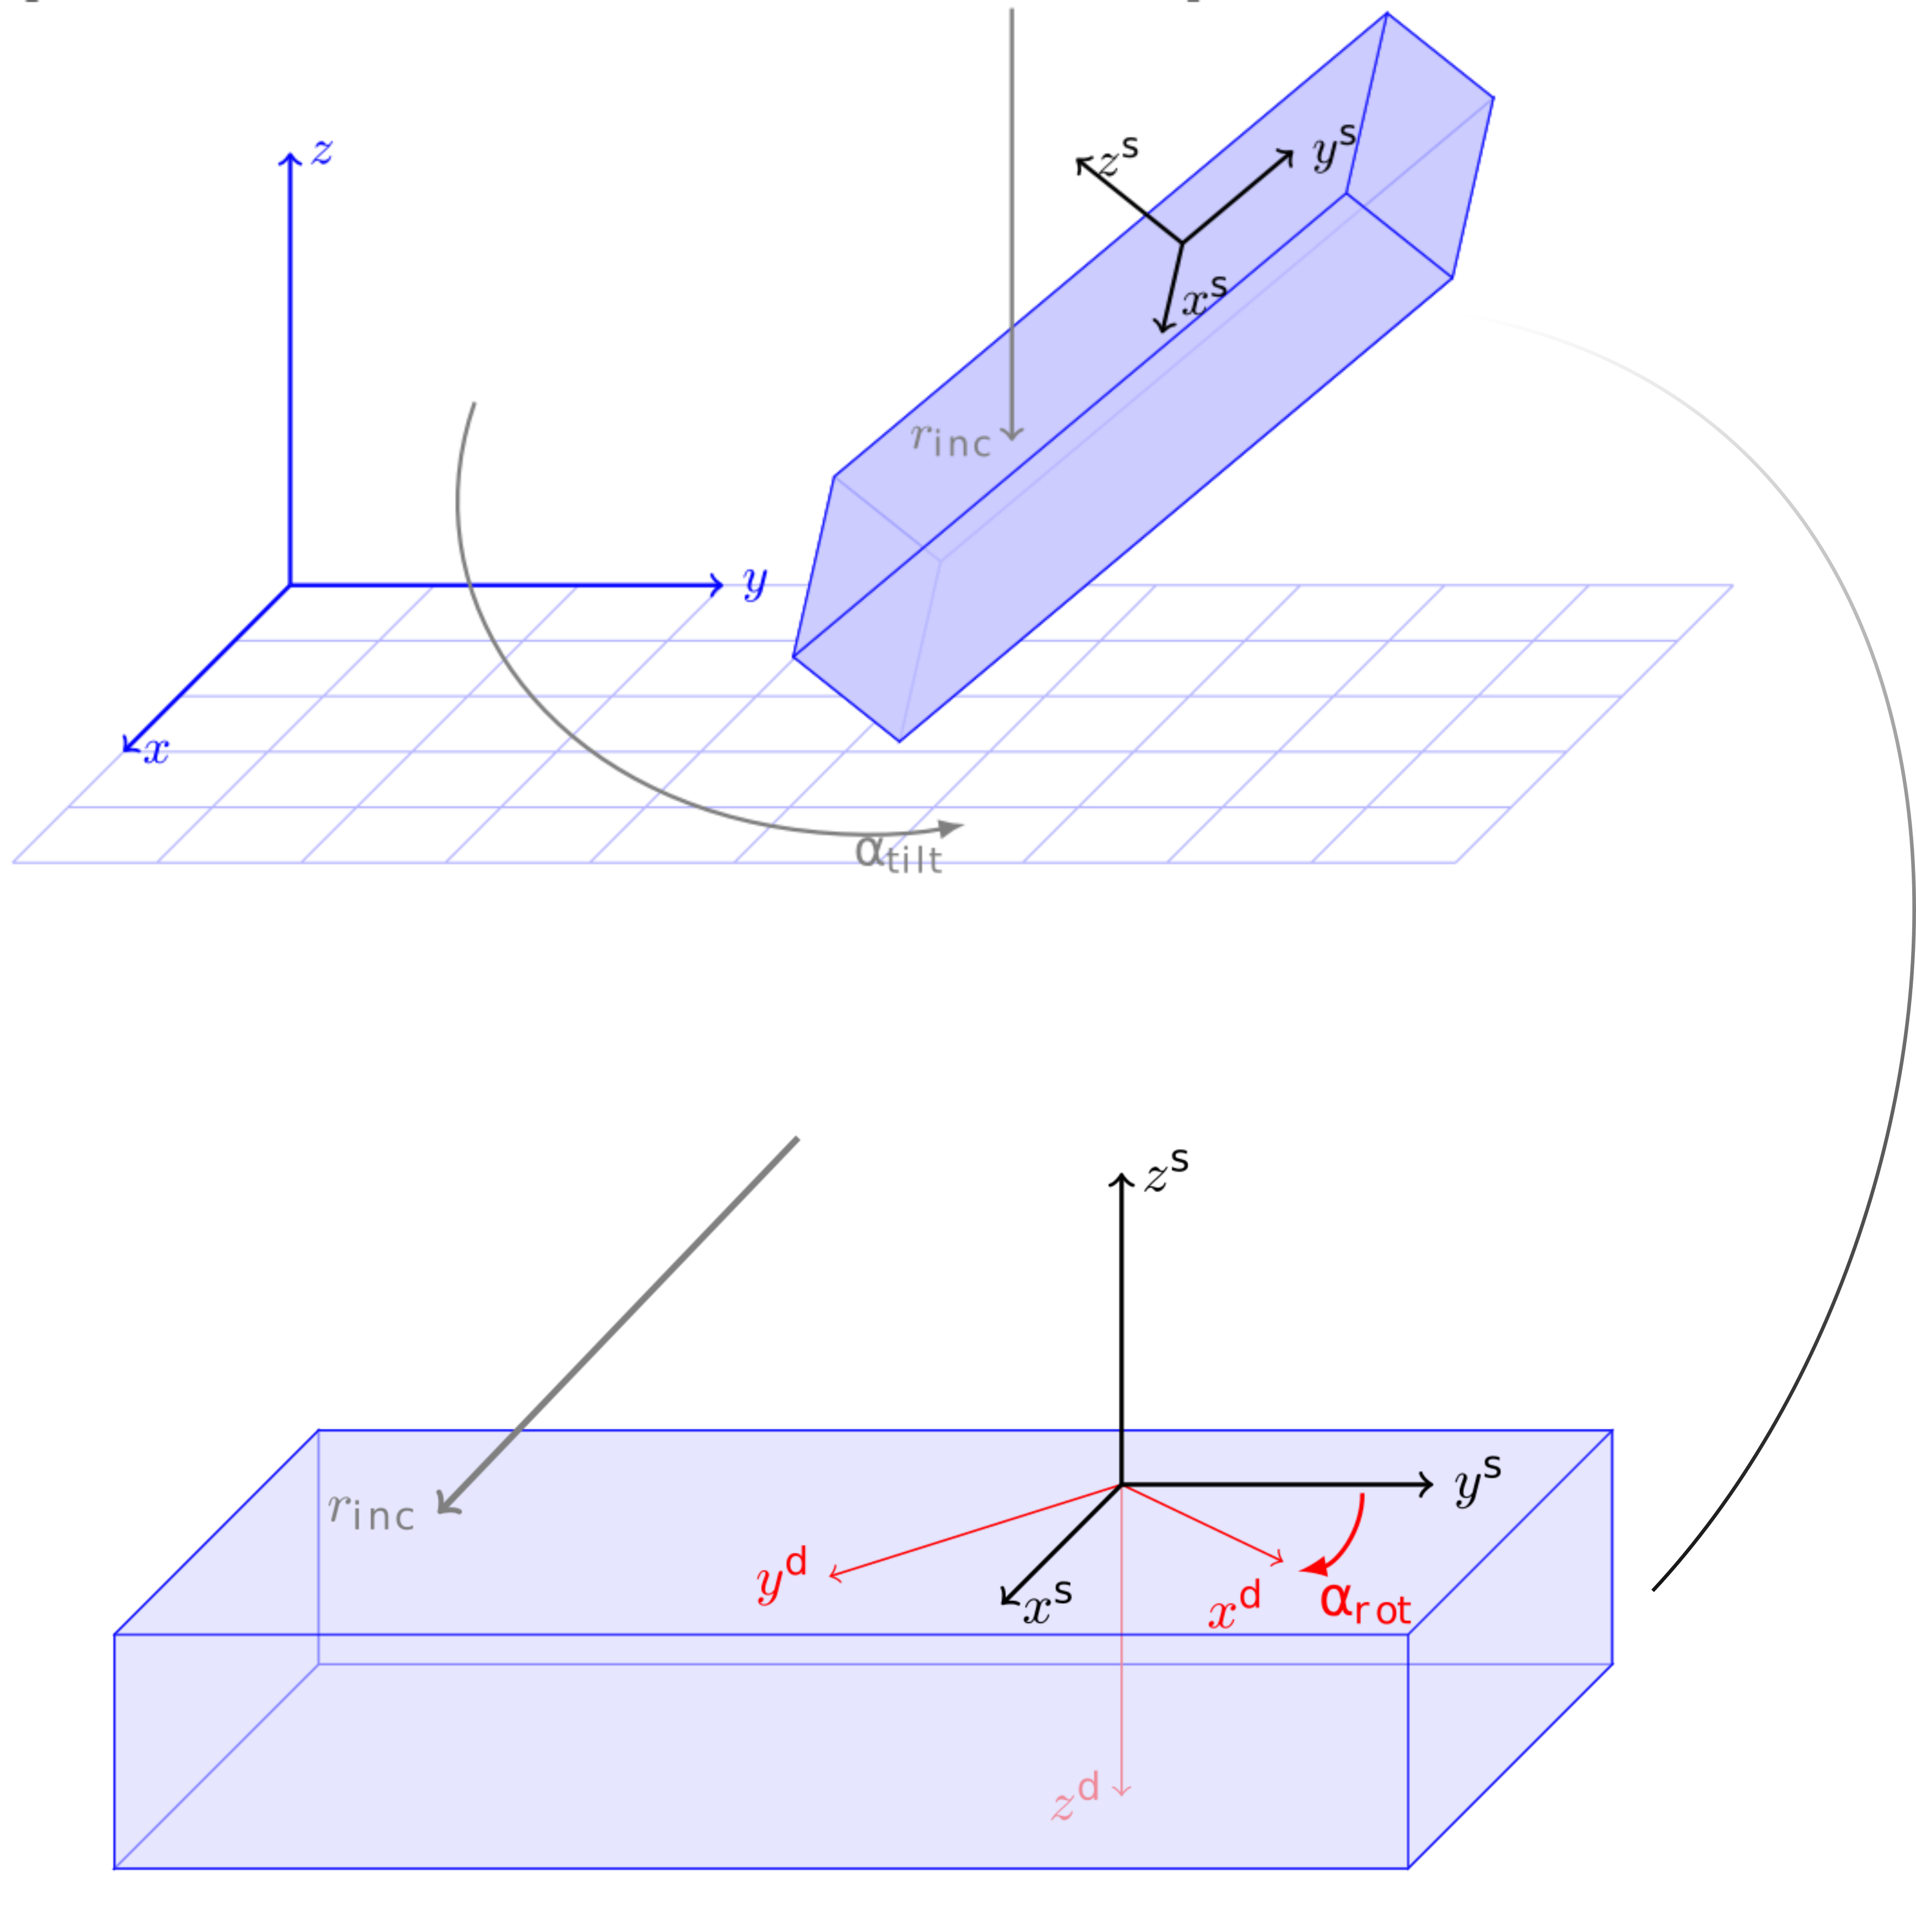
\includegraphics[width=0.78\linewidth]{Figures/calculus.png}
    \caption[Forward geometry reference frames.]{a) Tilted sample Cartesian frame (denoted by ($s$) and incident beam direction in the lab frame used here as a reference frame. b) Relationship between the dislocation reference frame (denoted by $d$) and the sample reference frame. The crystal frame is defined as an anticlockwise rotation along $z^s$ by $\alpha_{rot}$ and is not shown here.}
    \label{fig:sampleframe}
\end{figure}

If we define the coordinate frames used as meeting the following requirements:
\begin{itemize}
    \item the sample tilt axis is aligned with its $x$ axis as well as the lab $x$ axis;
    \item the crystal is non polar so that the crystallographic Cartesian $z$ can be aligned with the sample's $z$;
    \item the anticlockwise rotation from the sample frame to the Cartesian crystal frame along z is given by $\alpha_{rot}$;
    \item the dislocation line frame is defined as the right handed counterpart of the dislocation frame defined by
Tunstall~\cite{Tunstall64}, such that its $z$ axis is anti-parallel with the crystal frame and the sample frame $z$ axis,
\end{itemize}
then the transformation matrix from the dislocation reference frame to the sample reference frame can be written as:

\begin{equation}
    \mathcal{T}_{ds} = \mathcal{R}^z(\alpha_{rot}) \mathcal{R}^x(\pi) \mathcal{R}^z(3\pi/4)
\end{equation}
where $\mathcal{R}^w(\theta)$ is the anticlockwise rotation in a right handed coordinate system looking along $w$ by an angle $\theta$ as discussed on page~\pageref{subchap:basicRot}.

These transformations are implemented in this work using the \textit{ReferenceFrame} class from Python's
\textit{sympy.physics.vector} module~\cite{sympy} which proved useful in keeping track of the frames in which vectors and fields
are defined as well as the set of rotations between them. The total ECCI strain-like object is saved as a numerical
function of x, y, z position in a Python generated Fortran routine that will used later in the Howie-Whelan equations to calculate contrast. 

For these plots I had to split the work in multiple files and all can be found in the ``ecci-model'' folder on the GitHub repository: 
\begin{itemize}
    \item \texttt{geometry.py} contains crystallographic calculus for a cubic or hexagonal crystal.
    \item \texttt{coordinates.py} contains the relationship between the different reference frames.
    \item \texttt{calculateBeta2.py} calculates the beta function as an object dependent on the position from the dislocation, the tilt and rotation of the sample, the diffraction condition.
    \item \texttt{generateBetaModules.py} uses previous function to create Fortran callable modules containing the beta function.
    \item \texttt{plotField.py} is used to the displacement field.
    \item \texttt{plotStrain.py} is used for a number of plots for the strain profile.
\end{itemize}



%%%%%%%%     
\subsection{\texorpdfstring{$\beta$}{beta} isosufaces insights}
\label{sec:betacomparisons}
So far we have discussed the way to generate the strain components that affect the channelling contrast in the expression given in Eq.~\ref{eq:beta}. Since this parameter has the form of strain ($\partial u/ \partial x$), and, like the strain, it is dimensionless, I'm calling it here \textit{ECC-strain}. Since we also covered the grounds of calculating this value in different coordinate system it is useful now to observe its behaviour more closely.

For the following calculations and plots I am considering a \hkl[001] grown GaN sample containing TDs coming normal to the surface. The sample is tilted with respect to the incident beam. I am plotting isosurfaces, that is surfaces of constant $\beta$ value. Since it is common in this geometry for the ECC-strain to change sign around the dislocation (otherwise we would not have TD contrast), I plot both a positive $\beta$ value isosurface, analogous to compressive strain, in red and a negative value, analogous to tensile strain, in blue. In their absolute, the positive and negative $\beta$ values are chosen to be equal; I call them equidistant. Since the aim of this analysis is to observe the qualitative change in behaviour for different condition, for a series of images the $\beta$ values are the same. The off-white isosurfaces show the zero value positions. 


%%%%%%%%%
\subsubsection{Screw versus Edge TD isosurfaces}

There is insight that can be gained by looking at the shape of the strain components introduced by the threading dislocation in the Howie-Whelan two beam equations. I did that in Fig.~\ref{fig:edge} for an edge dislocation and   Fig.~\ref{fig:screw} for an screw dislocation in a GaN sample tilted at \SI{50}{degree}. Because strain is a three dimensional function it can be difficult to visualise, so what I did here is to plot only surfaces of constant strain component values (isosurfaces) both for a positive value (compressive strain) in red and a negative one (tensile strain) in blue, where the negative and positive values have the same absolute values. The isosurface values chosen are the same for the edge and screw dislocation.  The white cylinder in the middle indicates the position of the dislocation line which runs along the z direction. The red rod shows the projection of the diffraction condition vector \textbf{g}. The grey rod indicates the direction of the Burgers vector \textbf{b}, which is normal on the dislocation line for an edge dislocation and along the dislocation line, and here invisible, for a screw dislocation. 


A first observation to draw here is that in a highly tilted sample, the ECC-strain introduced by an edge TD will generally be larger than that introduced by a screw dislocation far away from the surface. This relates back to the discussion we had in Section~\ref{sec:tilteffect} on page~\pageref{sec:tilteffect} and has to do with unlocking larger strain components for an edge dislocation when tilting the sample. 



\begin{figure}[ht]
\centering
\begin{minipage}{.5\textwidth}
  \centering
  \captionsetup{width=0.8\linewidth}
  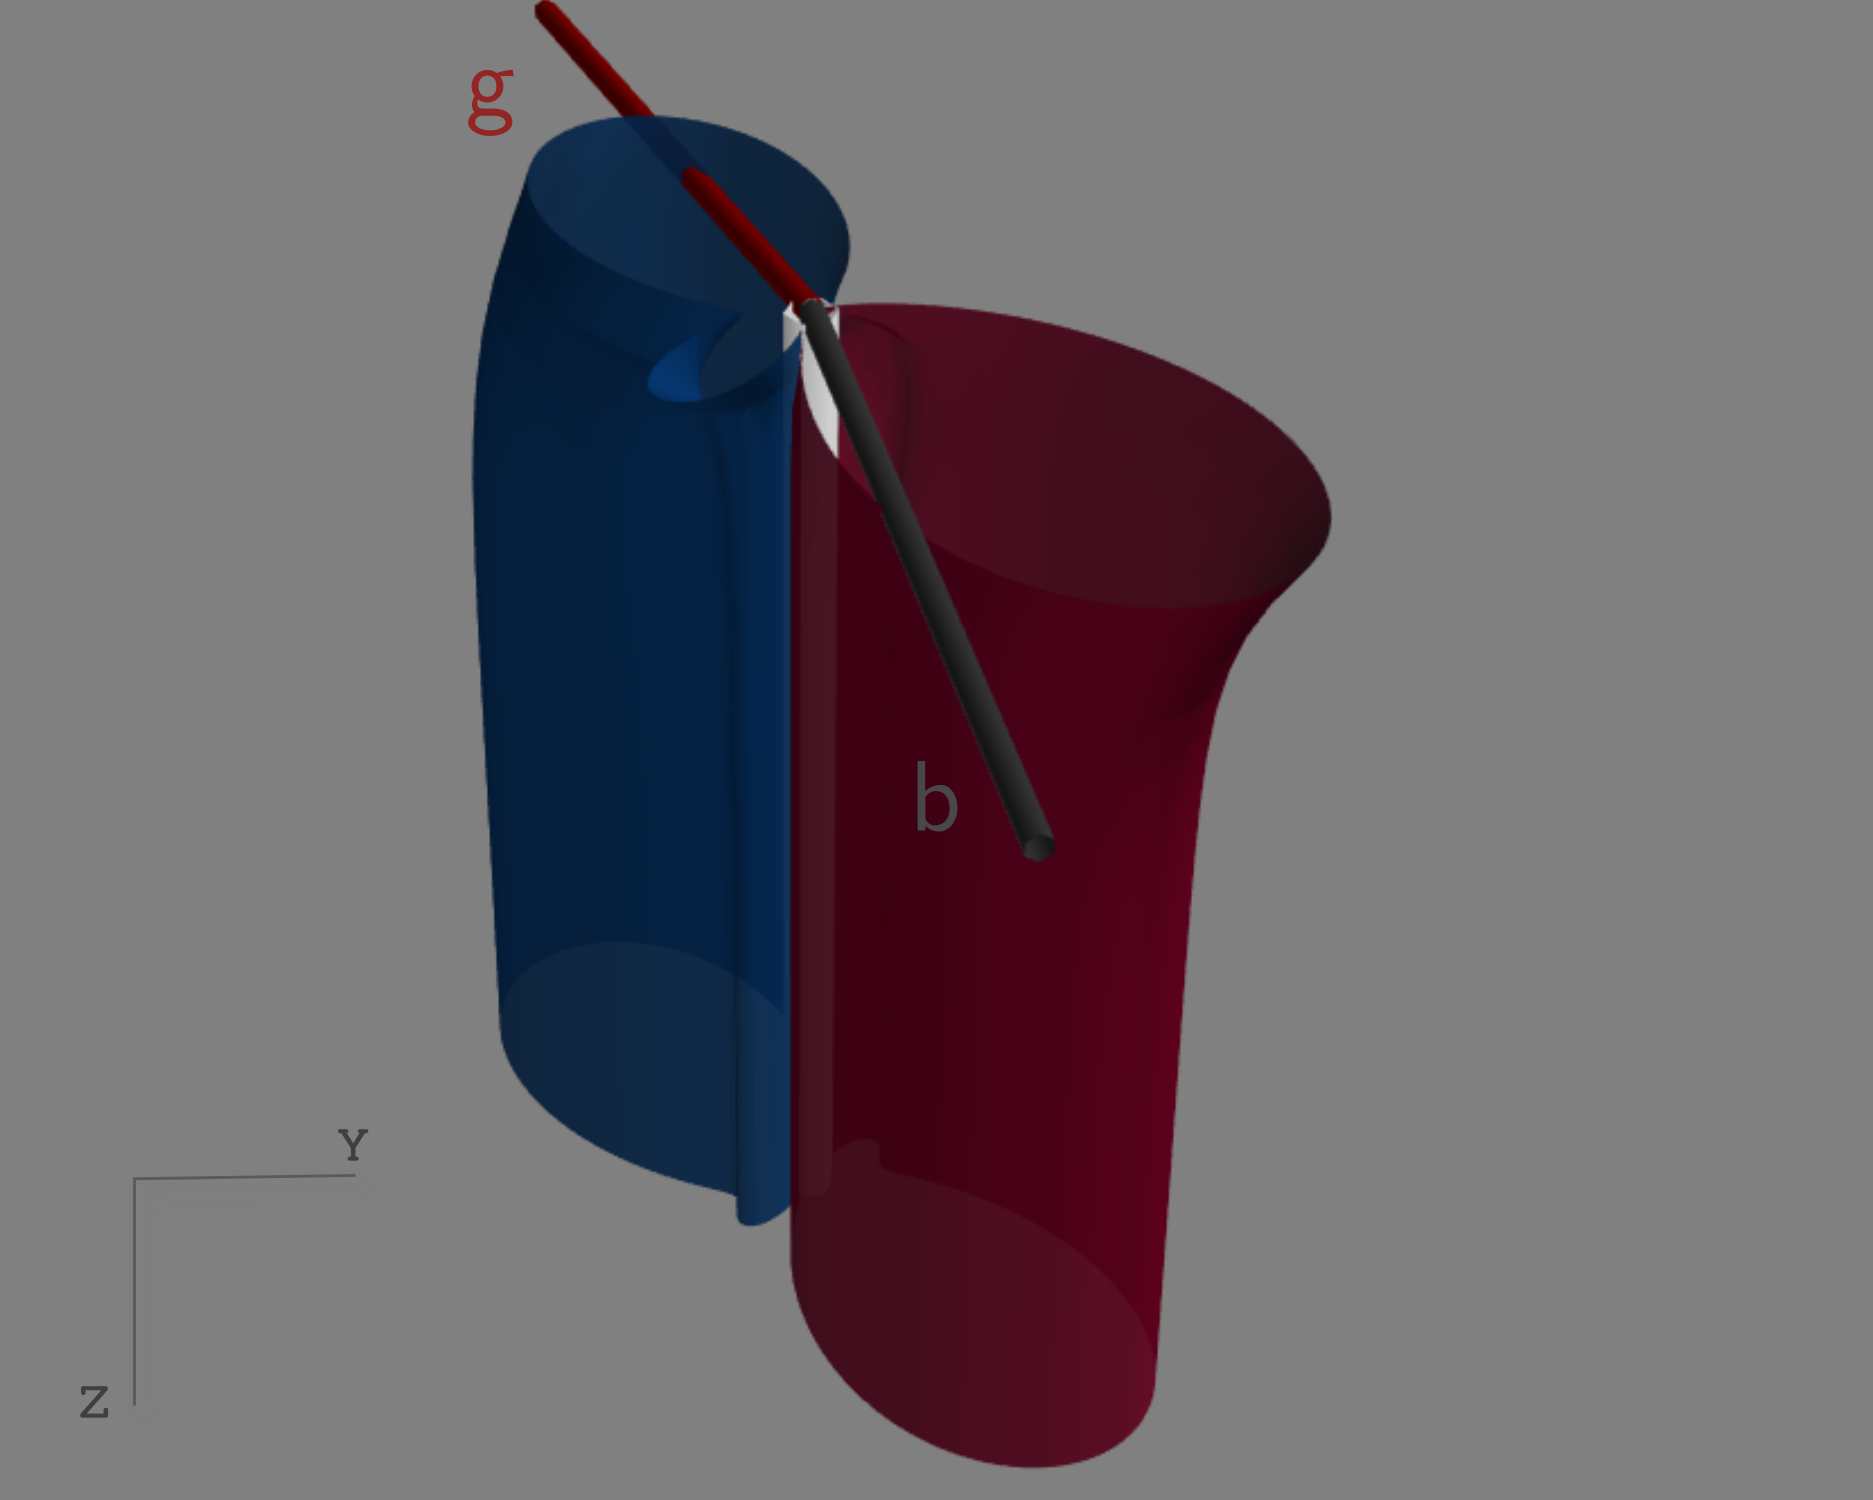
\includegraphics[width=.95\linewidth]{Figures/edge.png}
  \captionof{figure}{Edge TD ECC-strain field equidistant isosurfaces.}
  \label{fig:edge}
\end{minipage}%
\begin{minipage}{.5\textwidth}
  \centering
  \captionsetup{width=0.8\linewidth}
  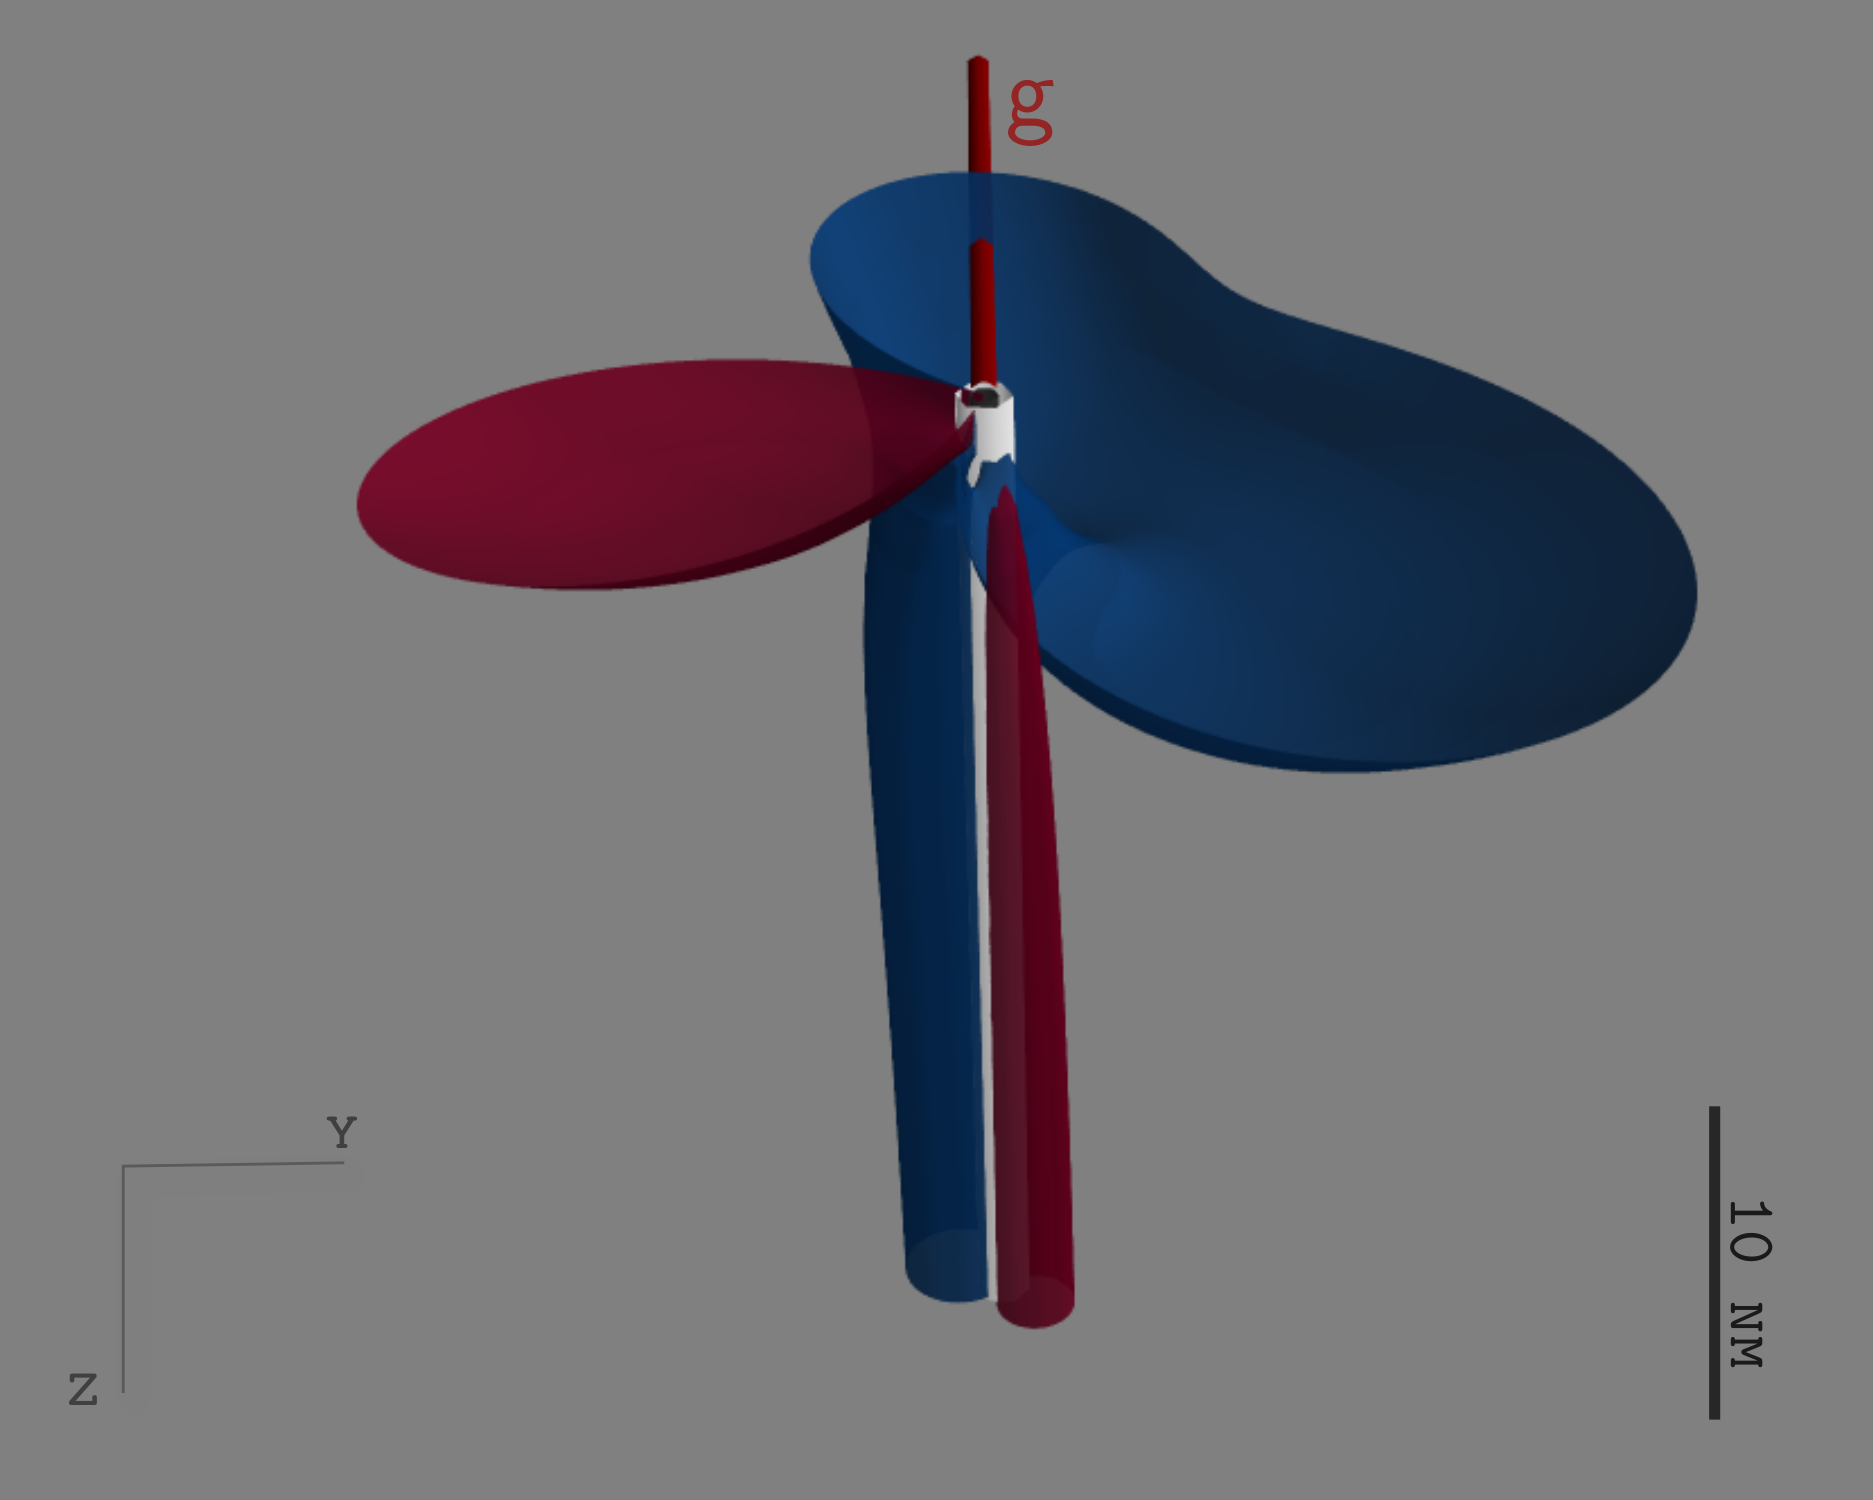
\includegraphics[width=.95\linewidth]{Figures/screw.png}
  \captionof{figure}{Screw TD ECC-strain field equidistant isosurfaces.}
  \label{fig:screw}
\end{minipage}
\end{figure} 




Another observation is that the surface relaxation affects ECC-strain of the two dislocation lines differently. At this high tilt there is little out of plane strain to relax for an edge dislocation and we can see the isosurfaces only curve a little at the top where the surface would be. The story is rather different for the screw dislocation in this specific diffraction condition. This time the isosurfaces make up large lobes close to the surface of the sample. Not only this, but we can observe an inversion of tensile-compressive strain as we follow the dislocation line to the surface. 

Since in the end we must integrate the two beam equations downwards in the sample, what we could take home from this comparison is that it will be probably more likely to observe edge dislocation contrast in the SEM. The screw dislocation ECC-strain becomes comparable in effect only close to the surface, therefore we expect the TD contrast to be comparable only when we are confident the diffracting beam penetration depth is only a few nanometers. 

%%%%%%%%%
\subsubsection{Mixed TD isosurfaces}

I want to quickly touch on how to predict mixed type dislocations. A mixed dislocation, in terms of continuum mechanics, is simply a linear combination of edge and screw displacement fields. It will come as no surprise that the ECC-strain will also look like a linear combination  of screw  and edge ECC-strain. This can be seen in Fig.~\ref{fig:mixed}.



\begin{figure}[ht]
    \centering
    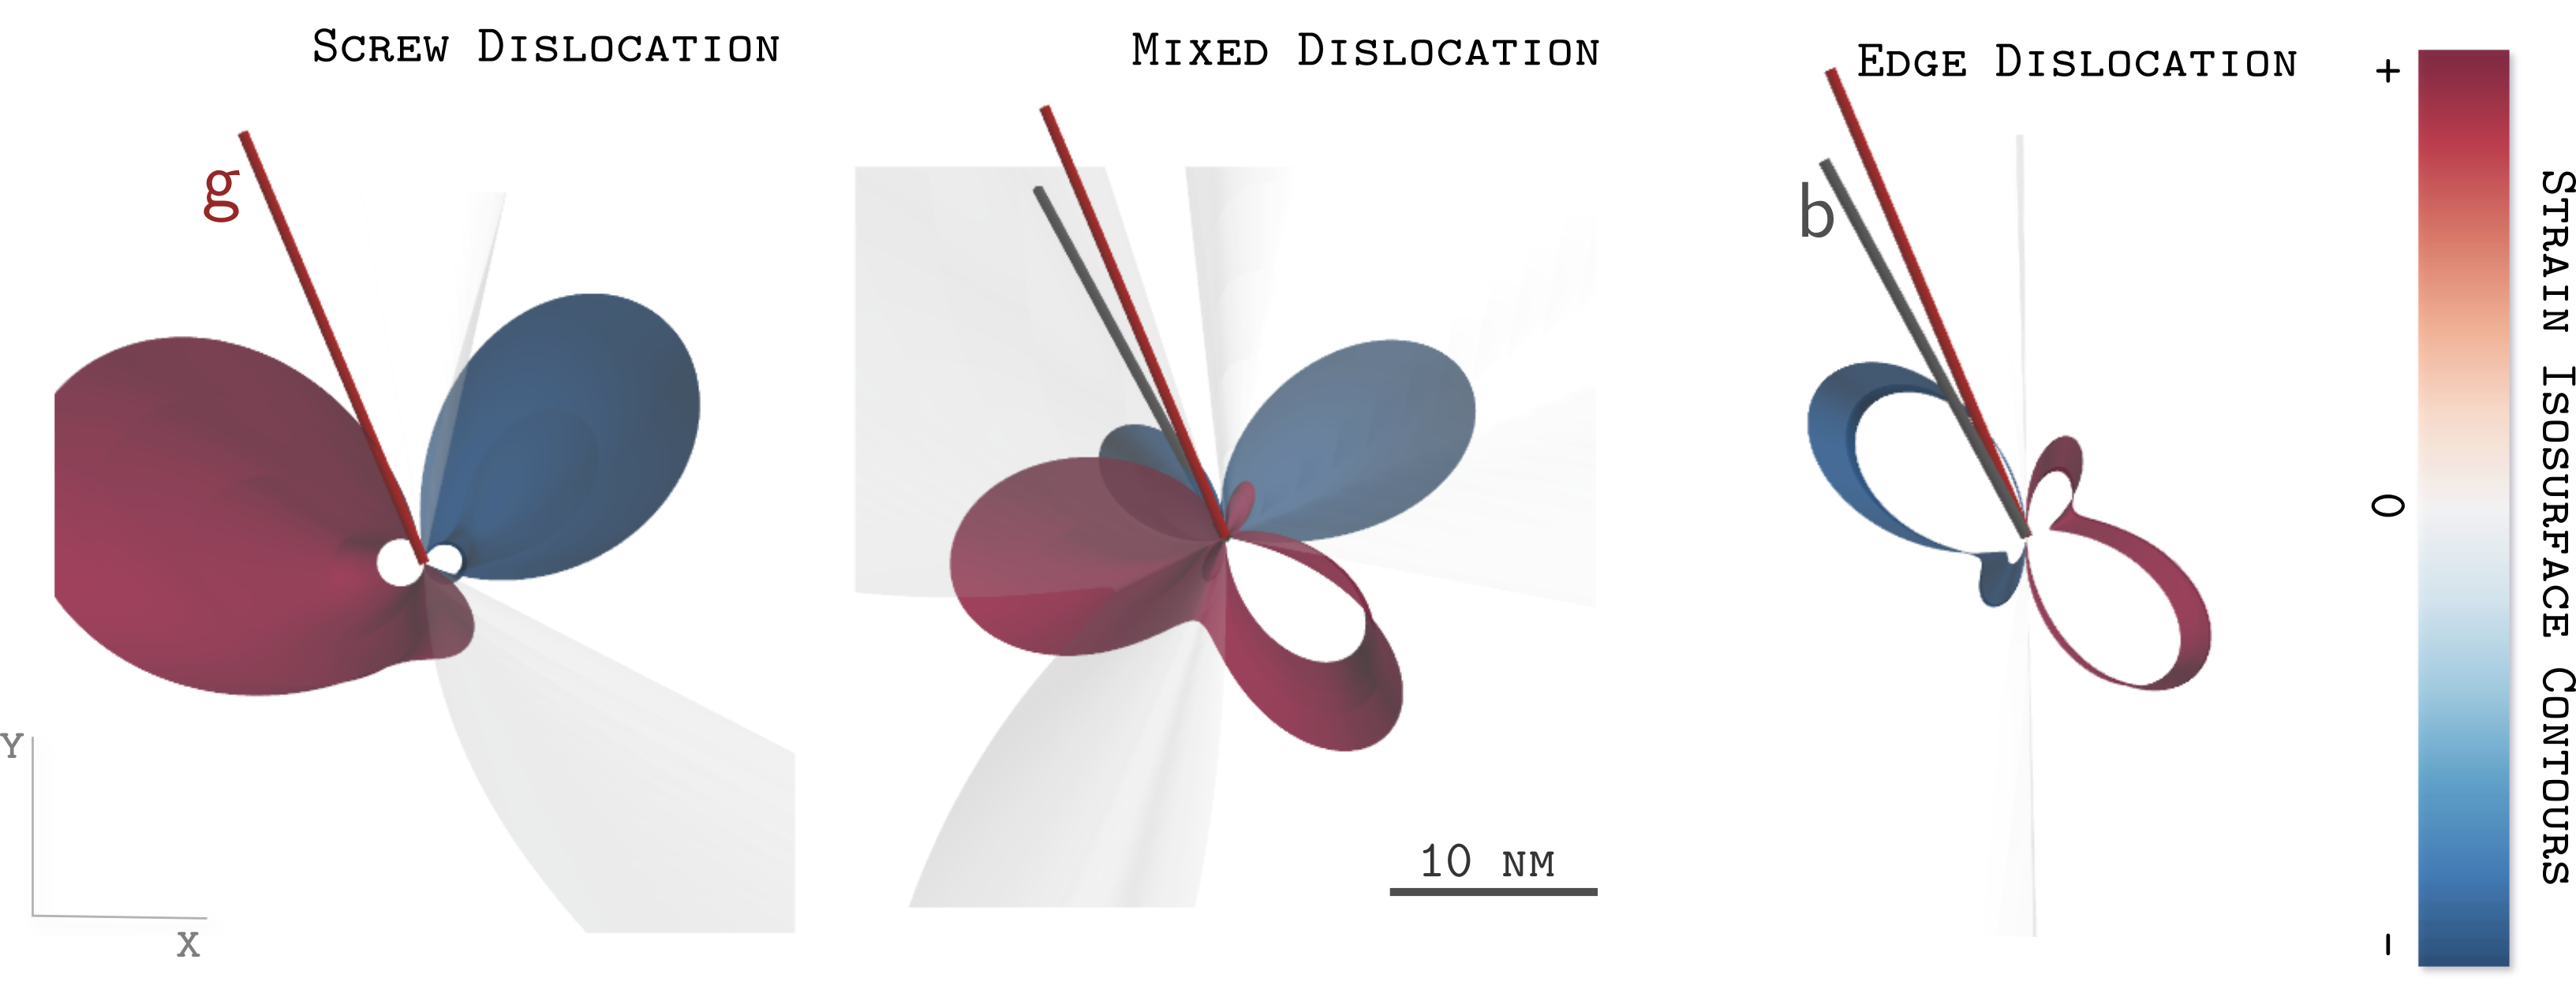
\includegraphics[width=1\linewidth]{Figures/GaNTDtop.png}
    \caption[Mixed TD ECC-strain.]{Top view of equidistant ECC-strain isosurfaces for a pure screw dislocation, a mixed and a pure edge dislocation, respectively in GaN. The sample is tilted at \SI{49.6}{\degree} and rotated by \SI{49.6}{\degree} such that \textbf{g}=\hkl[75-3] is available.}
    \label{fig:mixed}
\end{figure}


The large surface relaxation is inherited from the screw dislocation displacement field, however the profile is complicated by the edge TD components. For a deep diffracting beam penetration depth we would expect the ECC-contrast to resemble mostly the edge dislocation since it has the dominant strain contribution. 


Next, there is a critical question the channelling contrast literature is interested in: \textit{Is the orientation of the dark-white contrast affected first by the diffraction condition or by the Burgers vector?}

%%%%%%
\subsubsection{Dependence on \texorpdfstring{$\mathbf{g}$}{g}}
In Fig.~\ref{fig:gdependence} I show the top of the sample view of the ECC-strain isosurfaces for an edge dislocation in three different diffraction conditions. The red rods indicates the projection of the \textbf{g} vector and the grey rod shows the Burgers vector, \textbf{b}. I kept the set of planes, and therefore the magnitude of \textbf{g} the same, the red rods are projections and vary in size. 

Relating to the size of the projection of the \textbf{g} vector on the surface of the sample, the surface relaxation strain is larger or smaller. But the general geometry of the tensile-compressive strain, looking at the blue and red surface relaxation strain, does not seem terribly affected by which direction the reciprocal vector \textbf{g} points to. 

\begin{figure}[ht]
    \centering
    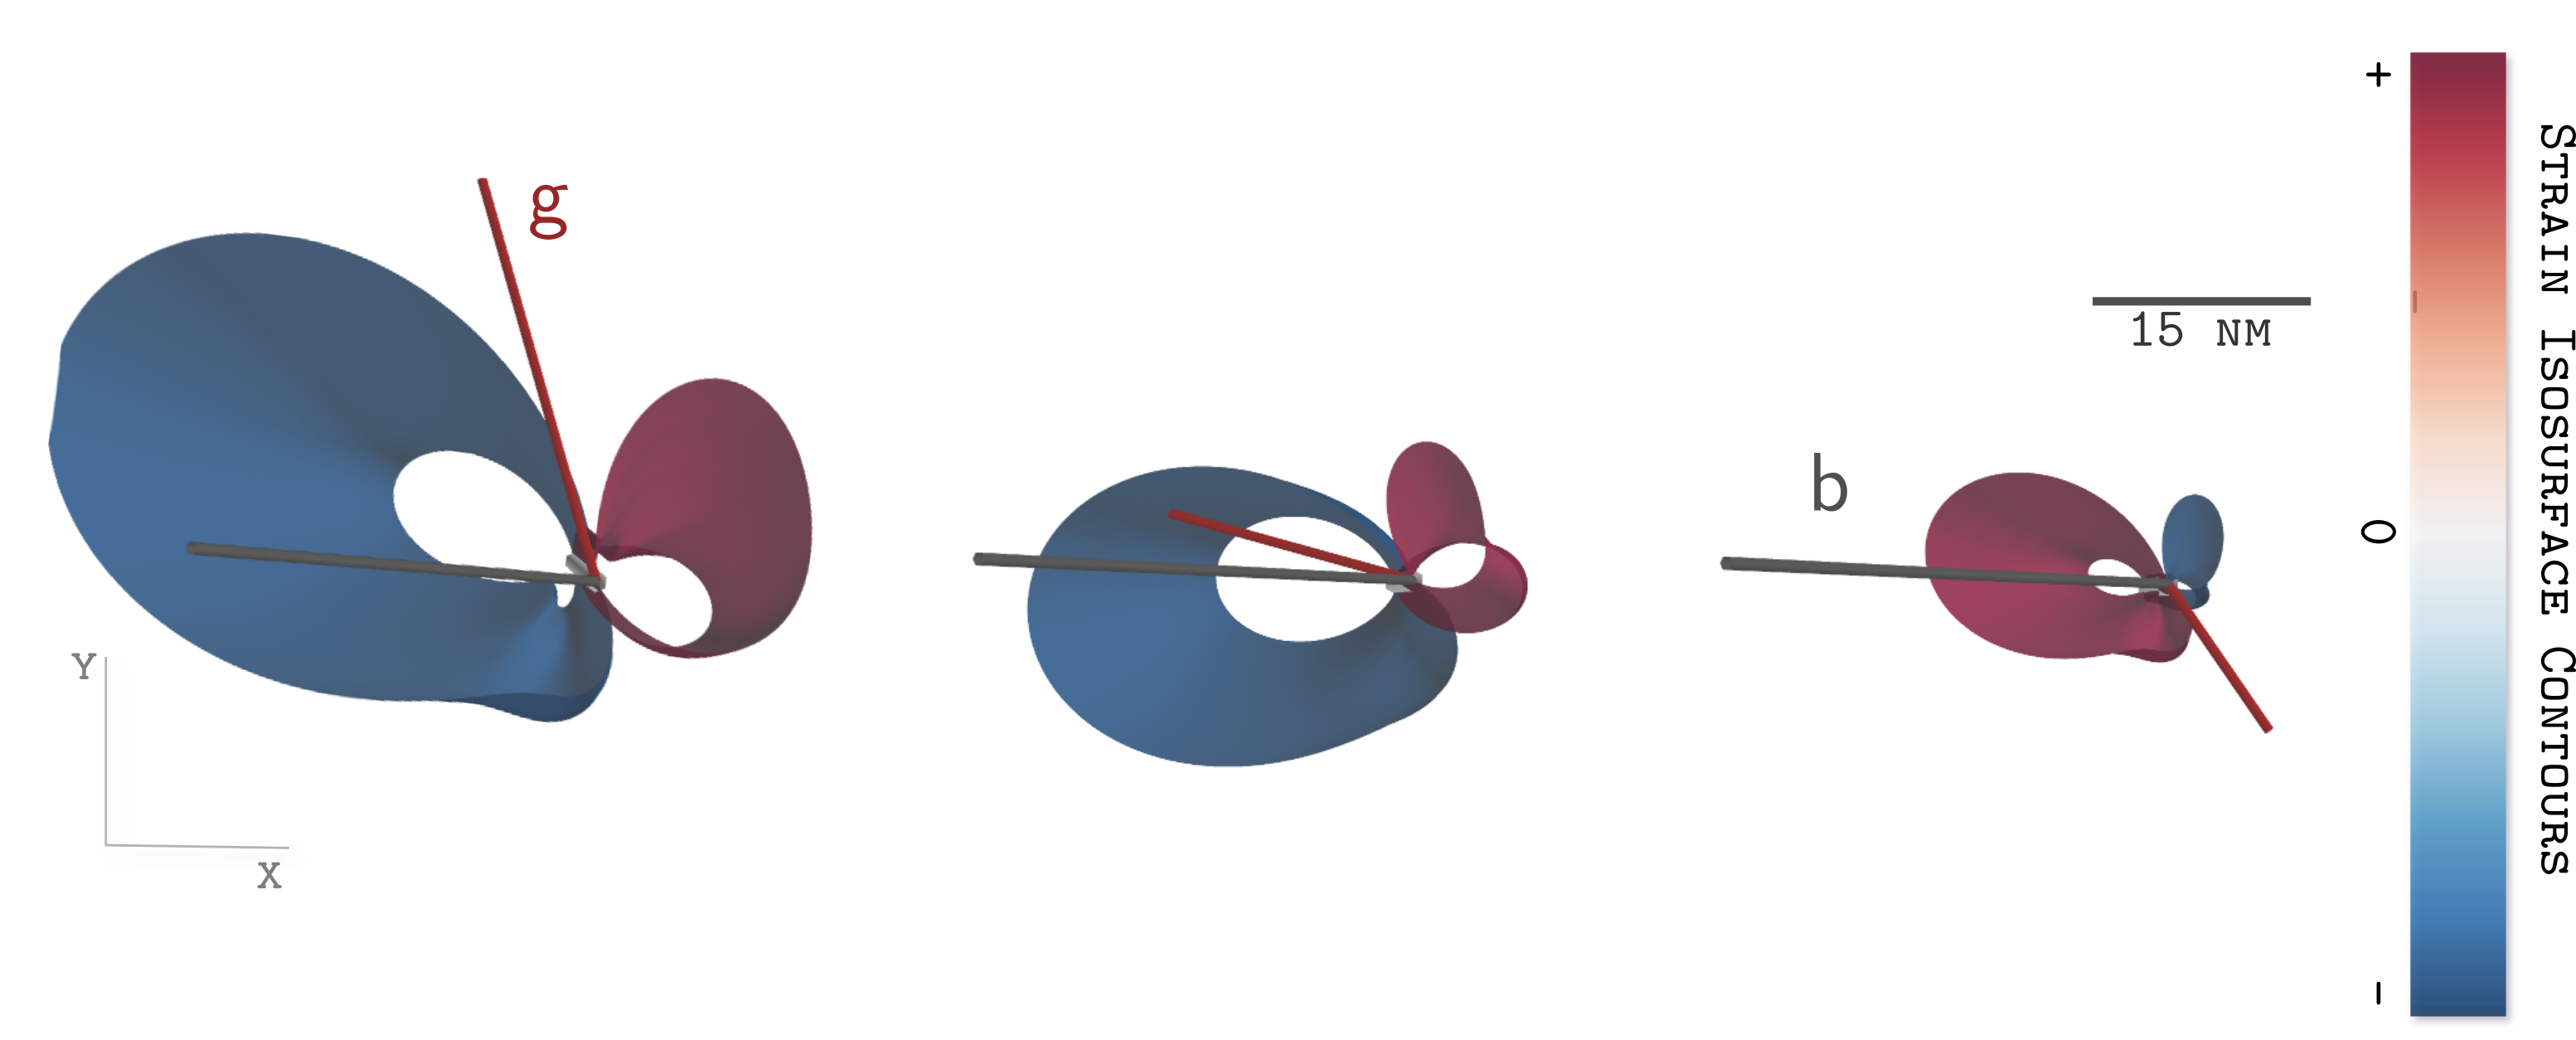
\includegraphics[width=0.95\linewidth]{Figures/gdependence.png}
    \caption[Edge TD ECC-strain in different orientations.]{Top view of equidistant  ECC-strain isosurfaces for a pure edge dislocation in different diffraction conditions given by the diffraction vector $g$ (red rod).  }
    \label{fig:gdependence}
\end{figure}

To emphasise this point in practice, Gunnar Kusch took two ECC images, Fig.~\ref{fig:gimportance},  from the same area of AlN in two different diffraction conditions shown in the bottom corner.   While the directions of the projected \textbf{g} vectors is different the black-white dislocation contrasts direction remains the same if only fainter. 

\begin{figure}[ht]
    \centering
    \includegraphics[width=0.95\linewidth]{Figures/gimportance.png}
    \caption{Forward geometry ECC image of AlN in two diffraction conditions shown by the ECPs inserts in the bottom corners.}
    \label{fig:gimportance}
\end{figure}
%%%%%%
\subsubsection{Dependence on \texorpdfstring{$\mathbf{b}$}{b}}

In Fig.~\ref{fig:bdependence} I show the top of the sample view of the ECC-strain isosurfaces for an edge dislocation in four different orientations of its Burgers vector.  The red rods, like before, indicate the projection of the \textbf{g} vector and the grey rods show the Burgers vector, \textbf{b}. The diffraction condition remains the same in the first three panels and for the last panel is flipped to -\textbf{g}. The off-white sections indicate the zero strain isosurface which looks complicated in the first panel.


\begin{figure}[ht]
    \centering
    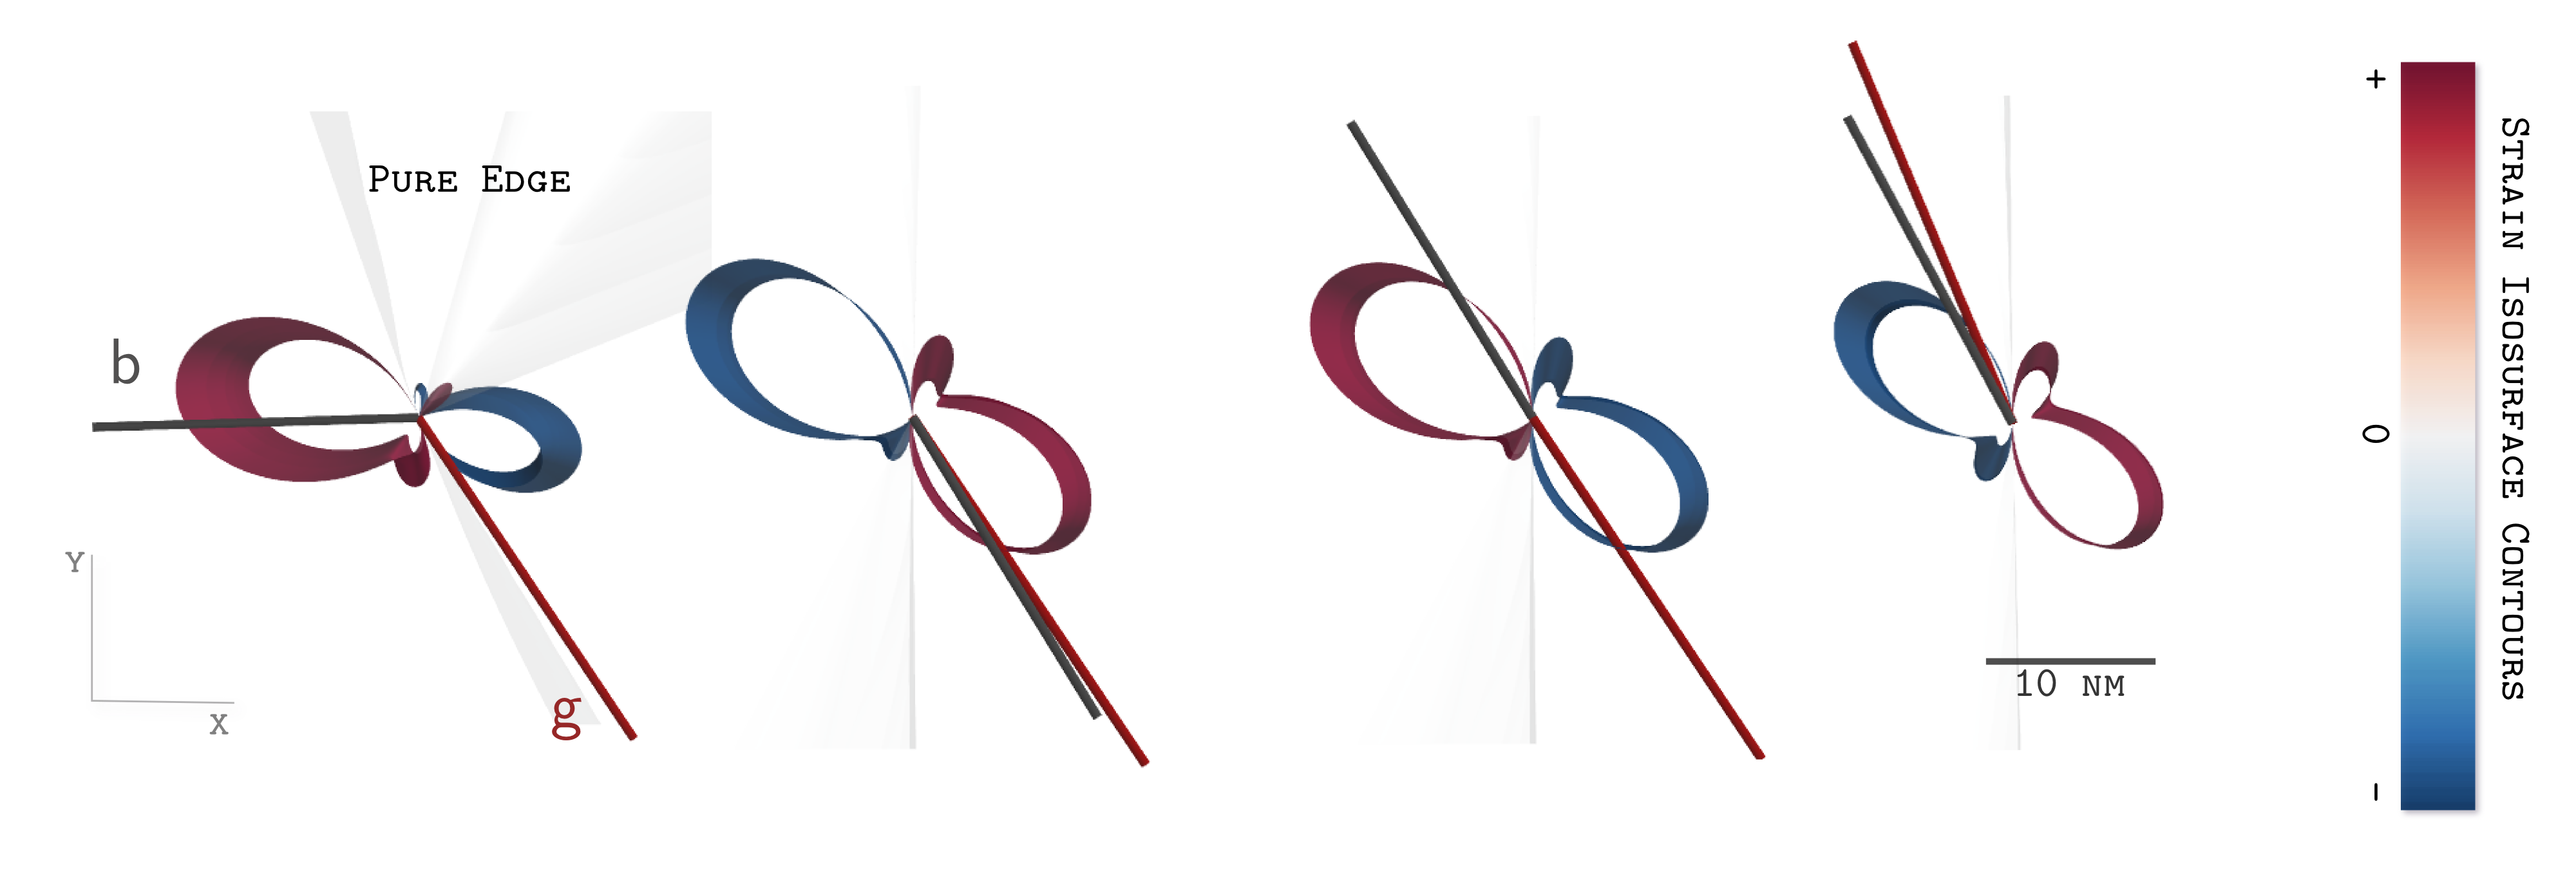
\includegraphics[width=1.05\linewidth]{Figures/bdependence.png}
    \caption{Top view of equidistant ECC-strain isosurfaces for a pure edge dislocation in different orientations indicated by the Burgers vector direction (grey rod).  }
    \label{fig:bdependence}
\end{figure}

Comparing the first two panels, where the Burgers vector, and essentially the dislocation, is rotated by about \SI{120}{\degree} in plane, we can observe that the tensile-compressive strain lobes rotate with \textbf{b}. Rotating the dislocation by \SI{180}{\degree}, what I did in panels two and three, perfectly flips the tensile and compressive strain. This is unlike rotating the sample, but, somehow, not the dislocation, by \SI{180}{\degree} in a system with mirror symmetry such that we can hit -\textbf{g}. I show this operation in panels three and four and while the  tensile-compressive strain lobes do flip, their shape is slightly changed. 

It is safe, therefore, to conclude that for the same diffraction condition the Burgers vector of an edge dislocation will dictate the ECC-strain geometry. This has been previously proposed by Naresh-Kumar \etal~\cite{Naresh}.



\pagebreak
%%%%%%%%%%%%%
\section{Backscattering event model}


For the backscattering process we follow the assumption made by Twigg \etal~\cite{Twigg09} that the contrast carrying signal comes from those electrons that leave the sample as soon as they suffer their first large angle scattering event, having previously suffered diffraction on their way in. The rest of the scattered electrons (making up the vast majority) will inelastically scatter multiple times on their way back out of the sample losing the contrast position information and only contributing to a uniform background. 

Twigg \etal~\cite{Twigg09} follows Rossouw \etal~\cite{Rossouw94}, analogously to the simulation of Kikuchi bands by Winkelmann \etal~\cite{Winkelmann07}, and integrates the beams wavefunctions over depth  to determine the probability of forward scattering at a certain penetration depth.  Rossouw \etal~\cite{Rossouw94}  approximate the cross-section for localised scattering events, $\sigma$, for independent partial Bloch waves $\phi^i$ to be:

\begin{equation}
    \sigma \approx A \sum_n Z_n^2 \sum_i | \phi^i(\tau_n)|^2 \exp{(-B_n}
\end{equation}
where the term $A$ is:
\begin{equation}
    A = \frac{2\pi N}{a_0^2 k^4} \frac{\cos{\beta_1} - \cos{\beta_2}}{(1-\cos{\beta_1})(1-\cos{\beta_2})}
\end{equation}
where $\beta_1$ and $\beta_2$ determine the minimum ($\beta_1$) and maximum ($\beta_2$) scattering angles allowed by the solid angle of the detector.

The BSE cross-section is proportional then to $P_n Z_n^2$ over all the atom sites in the volume of interaction, where $P_n=\sum_i |\phi^{(i)}(\tau_n)|^2$ is the probability density of electron backscattering from atom site $\tau_n$ smeared out by the Debye-Waller term $B_n$. 

The trick now is to calculate the Bloch waves contributions in the equations above. Luckily we have the two beam differential equations~\ref{eq: multiDHWTD} from which we could (we will see in next section how) calculate the intensities in the direct and diffracted beams. The columns approximation electron beams and electron Bloch waves are equivalent descriptions of the electron wavefunction in the crystal~\cite{Howie61}:

\begin{equation}
\begin{split}
    \Psi(\mathbf{r})  = & \sum_i \alpha^{(i)} \phi^{(i)} =  \sum_i \alpha^{(i)} \sum_{\mathbf{g}} C_{\mathbf{g}}^{(i)} \exp(2\pi i \, (\mathbf{k}^{(i)}+\mathbf{g})\cdot \mathbf{r}) \\
                  = & \sum_{\mathbf{g}} \psi_{\mathbf{g}}(r_{inc}) \, \exp(2\pi i \, (\mathbf{\hat{r_{inc}}} + \mathbf{g})\cdot \mathbf{r})\\
\end{split}
\end{equation}


The first line is the electron wavefunction inside the as superposition of Bloch waves of amplitudes  $\alpha^{(i)}$ and partial Bloch waves components $\phi^{(i)}$, and the second line is in terms of beams for every diffraction condition $\mathbf{g}$. Note that in the equation above the wavefunction is given in terms of the position vector $\mathbf{r}$ which needs to be replaced by the atoms positions $\tau_n$ for the probability computations. 

The probability distribution function in terms of two beams is then:
\begin{equation}
    |\Psi(\mathbf{r})|^2 = |\psi_0 \exp(2 \pi i \, \mathbf{r_{inc}}\cdot \mathbf{r}) + \psi_g \exp(2 \pi i \, (\mathbf{r_{inc}+\mathbf{g}})\cdot \mathbf{r})|^2
\end{equation}
Note that both the direct and diffracted beam(s) contribute to the contrast and their backscattered cross sections and probabilities must be computed separate and added together thorough the equation above to calculate the total BSE contribution.
 


Twigg and Picard~\cite{Twigg09} used a slightly different approach, yielding very similar contrast predictions results. They assumed that the localisation of the backscattering process is implicit in the imaginary potential used to treat absorption. Therefore, they integrate the beam intensities along their path in order to calculate the probability of backascattering.  


%%%%%%%%%%%%%%
\section{ Numerical simulation of electron diffraction model}
\label{sec:numerical}
The dislocation line is placed in the centre of a square mesh. The pixels on the mesh are populated by columns aligned parallel to the incident beam and of length equal to the electron beam penetration depth. The HWD differential equations are then solved numerically step-wise for each column taking into account the variation of the displacement field along the column calculated previously. We use the Runge-Kutta algorithm available in the \textit{zvode} library~\cite{Hindmarsh85} for the numerical integration which, even for stiff equations, can calculate the entire mesh in seconds when using a modern computer.

With the electron beam wavefunction numerically solved, I then ``integrate along the beam'' by summing up their squared values for the decided penetration depth. I then calculate for all the species in the sample the BSE cross section and the total BSE contribution for a pixel. After the backscattering event the electrons heading towards the detector are projected by yet another coordinate transformation on its surface.

\begin{figure}[ht]
    \centering
    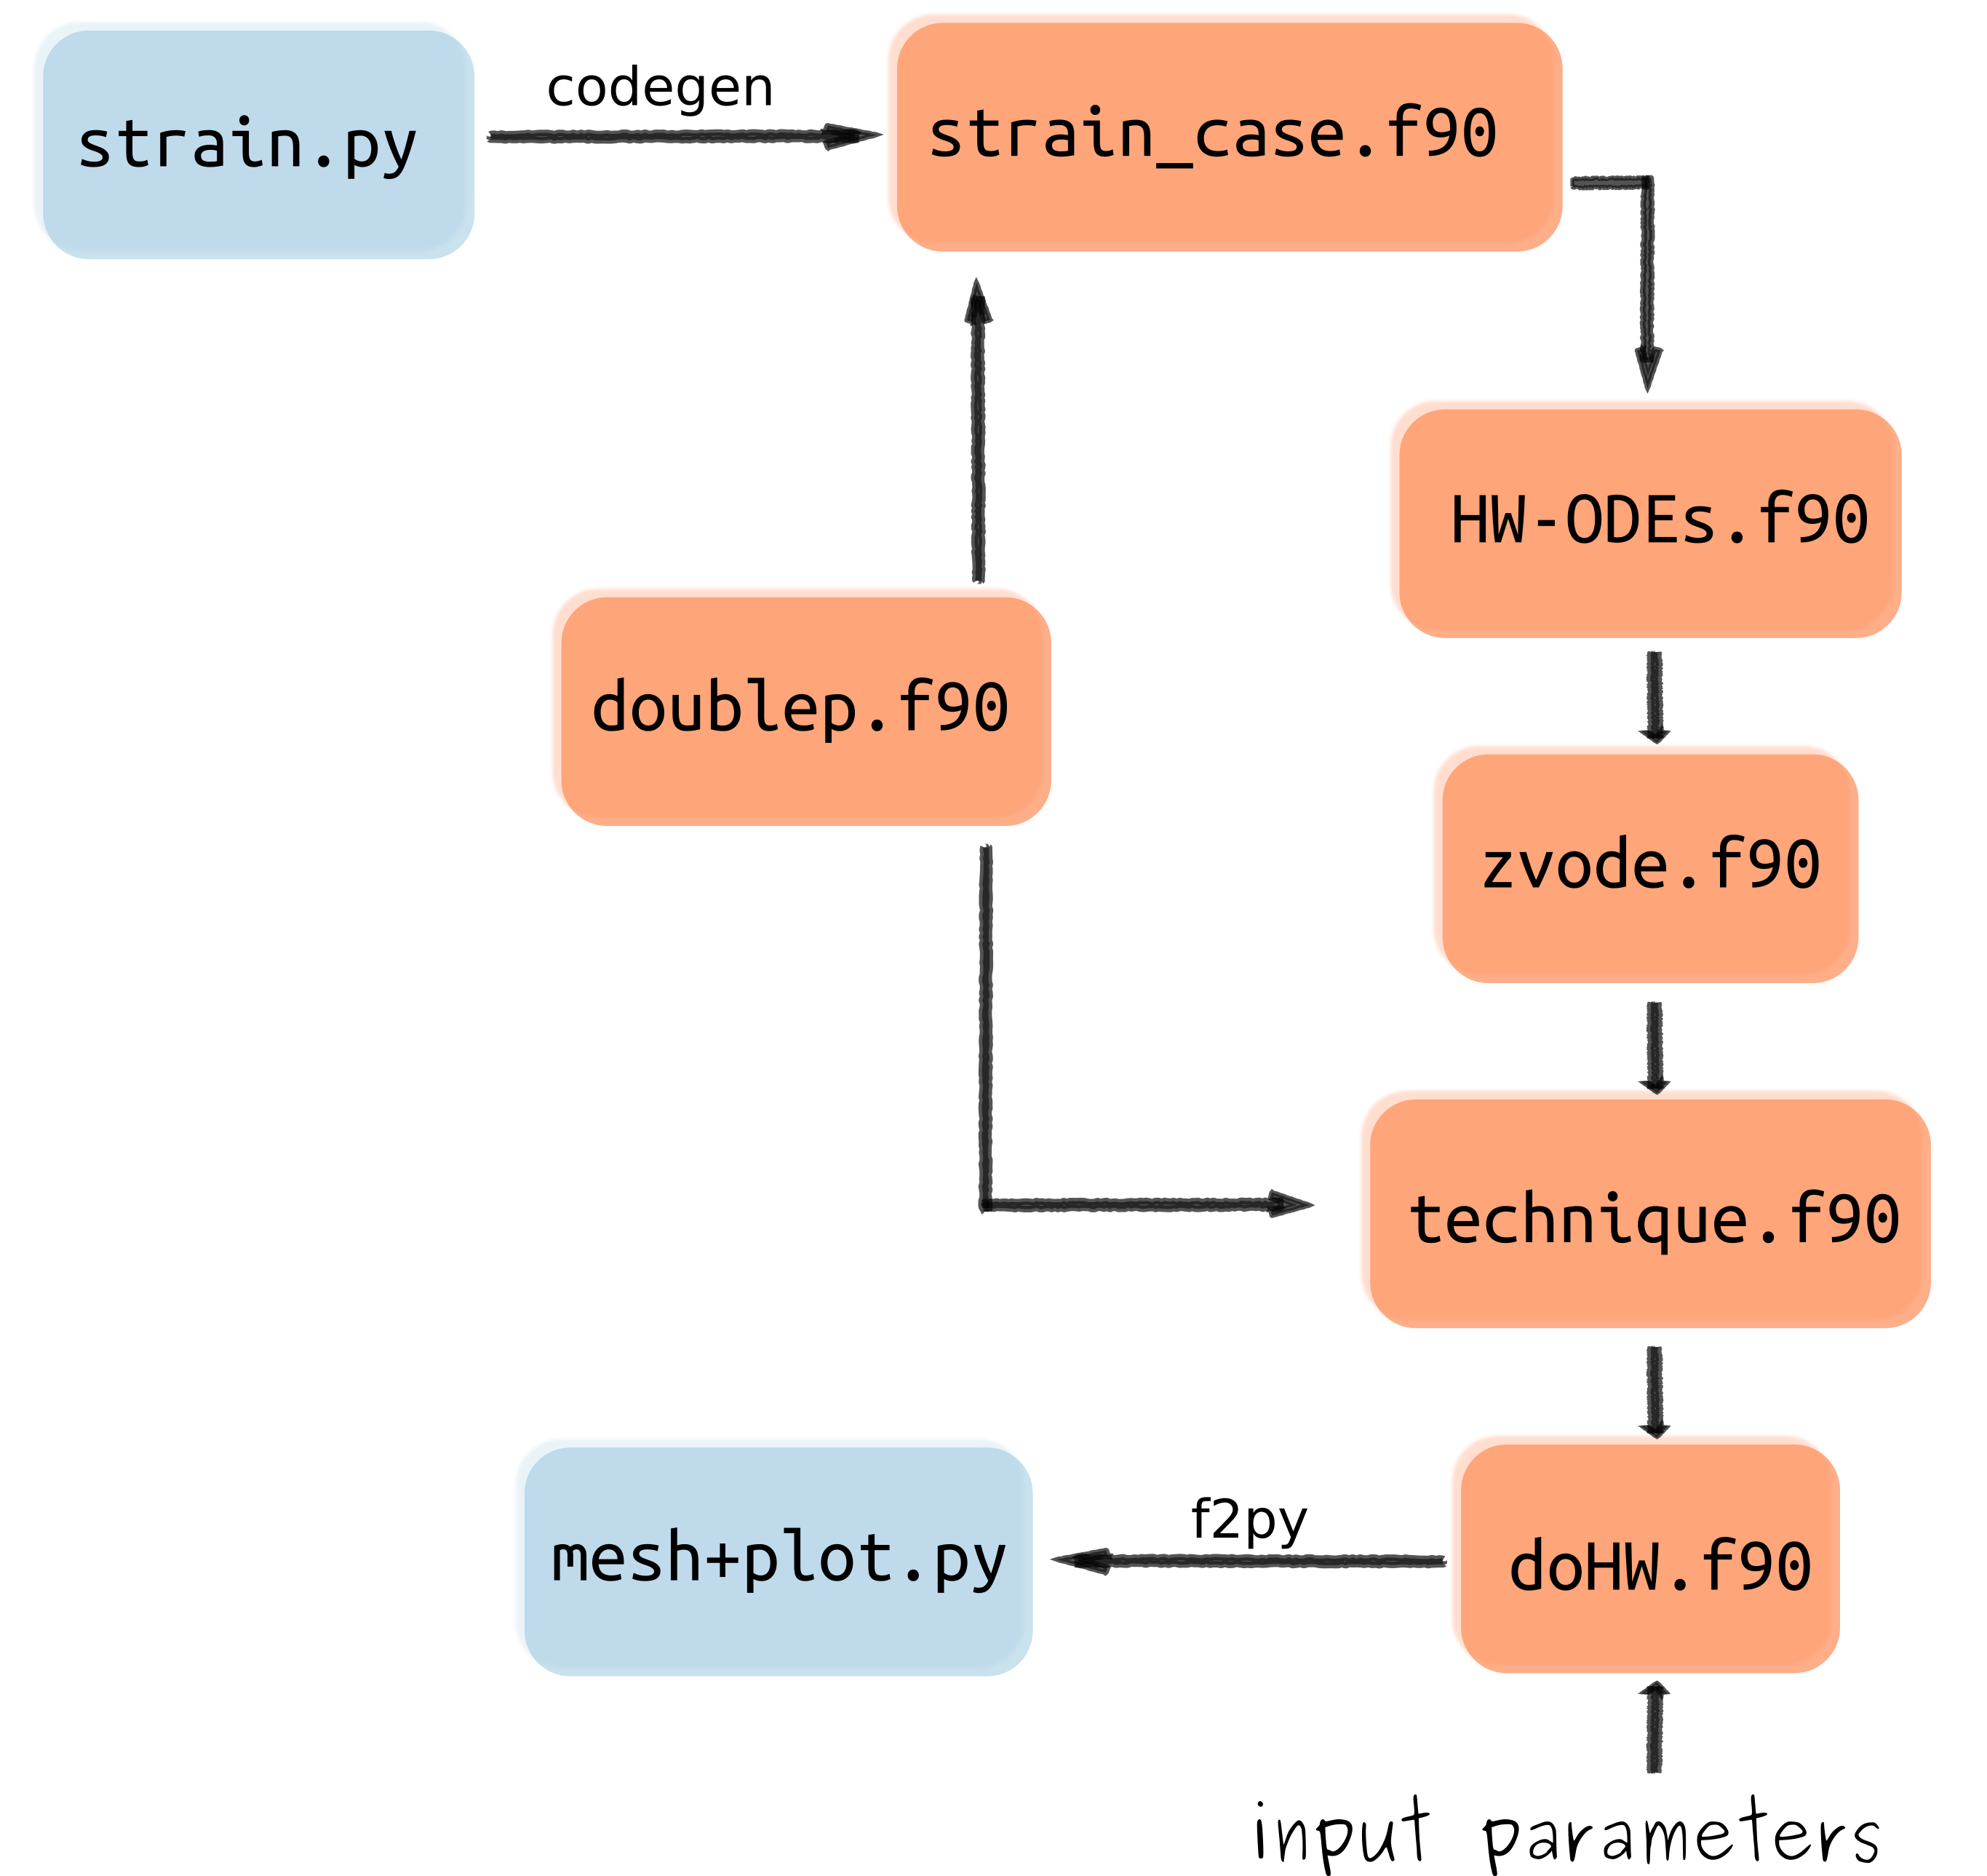
\includegraphics[width=0.6\linewidth]{Figures/code.png}
    \caption{ The code structure  schematics for predicting TD contrast in ECCI . }
    \label{fig:code}
\end{figure}

The full code I used can be found in  the ``ecci-model'' folder on the GitHub repository. The Howie-Whelan two beam integration is not particularly easy  to read, neither is the backscattering process. I hope one day to make it readable, but until then, the schematics of it is shown in Fig.~\ref{fig:code}. I calculate the ECCI strain for each specific geometry and diffraction condition using Python and generate the long, unsimplifiable three dimensional numerical $\beta$ function. These functions are turned to Fortran readable modules using the \textit{codegen} function. Eventually, the $\beta$ functions are fed into the Howie-Whelan ODEs, which are then integrated column-wise on a 2D mesh using the \texttt{zvode} library. There is an option to compare a TEM prediction to the ECCI one.   The main file is \texttt{doHW.f90} which also contains all the hard-coded GaN parameters, the depth of integration and the sample area considered. I wrote a \textsc{Makefile} to control all of this. In the end, I obtain a file containing a two dimensional contrast function which could be plotted, for instance using more Python. 



%%%%%%
\section{Contrast predictions in GaN}
\label{sec:contrastGaN}
Dislocation analysis of GaN cross sections in TEM shows that the TDs predominantly show pure edge character with the dislocation line lying along the crystallographic $c$ axis and the Burgers vector pertaining to the family  1/3\hkl<11-20>~\cite{Hino00}.

The ECC images of these types of TDs in the forescatter geometry, with the film tilted at a high angle, will sample strain components which are not parallel to the dislocation line. While the plan view TEM images show TD black-white contrast being aligned perpendicularly to the  Burgers vector of the dislocation, the geometry of the ECCI highlights a different set of strain components which can align the contrast direction along the Burgers vector.

In Fig.~\ref{fig:rotateEdge} I show possible strain profiles sampled in a sub-surface plane parallel to the top of the film (similar to Fig.~\ref{fig:tilting} for three geometries of orientation of \textbf{b} with respect to \textbf{g}. In Fig.~\ref{fig:rotateEdge} a) and c) the maximum variation in strain is aligned with the direction of the Burgers vector. The image in Fig.~\ref{fig:rotateEdge} b) shows a quasi-invisibility (drastic reduction in strain variation) criterion when the infinite-lattice dislocation strain component dominates, in particular in the case when vector \textbf{g} is perpendicular to the Burgers vector~\textbf{b}.

\begin{figure}[ht]
    \centering
    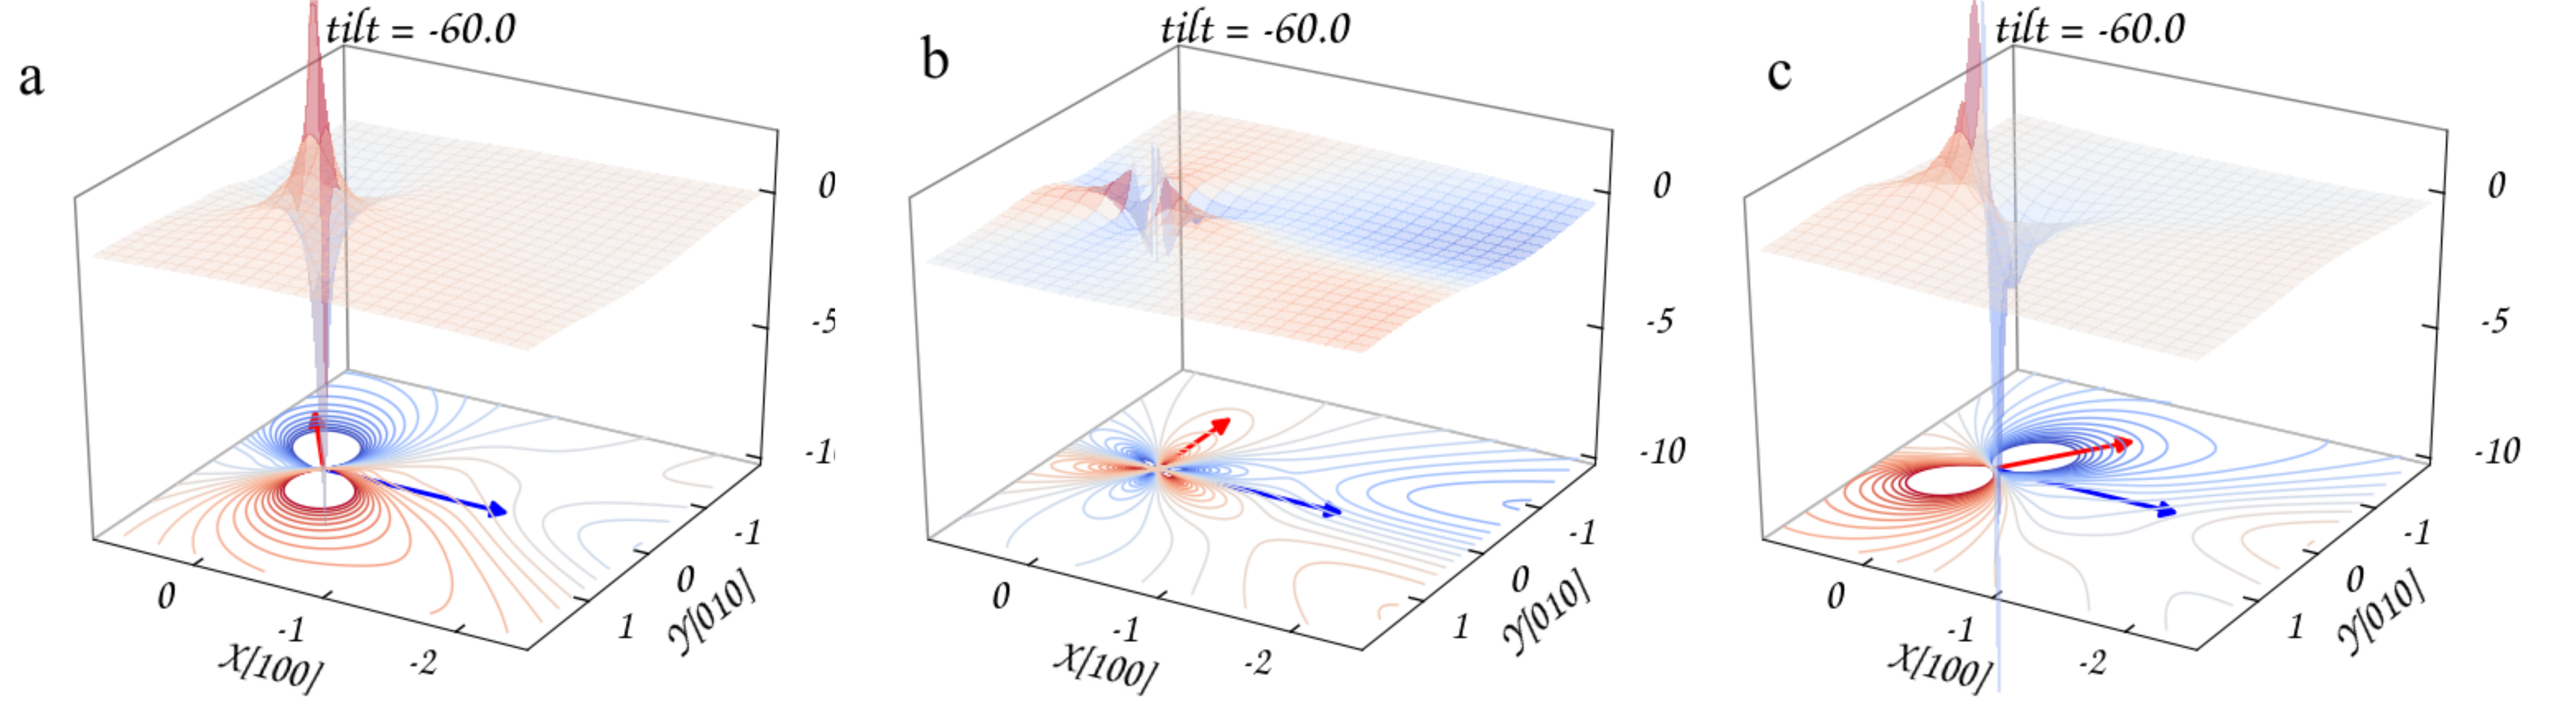
\includegraphics[width=1.1\linewidth]{Figures/rotateEdge.png}
    \caption[Edge TD ECC-strain in different orientations.]{Accessible strain profiles for an edge TD in wurtzite GaN sampled in a plane parallel  to the surface and \SI{1}{\nano \meter} below the interface. The sample is tilted  \SI{60}{\degree} from the original horizontal position. The marked red and blue arrows show the direction of the Burgers vector projection and the direction of the projection of \textbf{g}, respectively. Vector\textbf{ g} remains the same across the three images while vector \textbf{b} is rotated in  increments in the same plane such that the angle between the vectors is: a) \SI{30}{\degree}, b) \SI{90}{\degree}, c) \SI{150}{\degree} }
    \label{fig:rotateEdge}
\end{figure}


\label{Naresh}
Two beam plan view ECC images were acquired by Naresh-Kumar~\cite{Naresh} using a \SI{50}{\degree}  sample tilt together with electron channelling patterns from the same area for two different crystal rotation: $\mathbf{g}_a$ =\hkl[-5-7-3] and $\mathbf{g}_b$ =\hkl[75-3]. This was achieved by tilting the crystal in plane with about \SI{3}{\degree}. The electron beam energy was \SI{30}{\kilo \electronvolt}. The same small area from the two images is shown on the left in Fig.~\ref{fig:contrast} a) and b) with the predicted dislocation contrast for three different possible Burgers vectors shown on the right. From the qualitative comparison we can determine which dislocations show similar behaviour to the model cases and assign Burgers vectors.

The modelling parameters used here are shown in the Table~\ref{Table:params}. The extinction distances are calculated numerically from the Fourier coefficient of the electrostatic potential of the crystal. The scattering factors of this potential are calculated using Weickenmeier-Kohl parametrisation as implemented in EMsoft~\cite{EMsoft}. For the beam penetration depth calculation needed for the estimation of the diffraction columns integration depth we made use of a continuously slowing down inelastic scattering Monte Carlo model~\cite{casino}. 






\begin{figure}
    \centering
    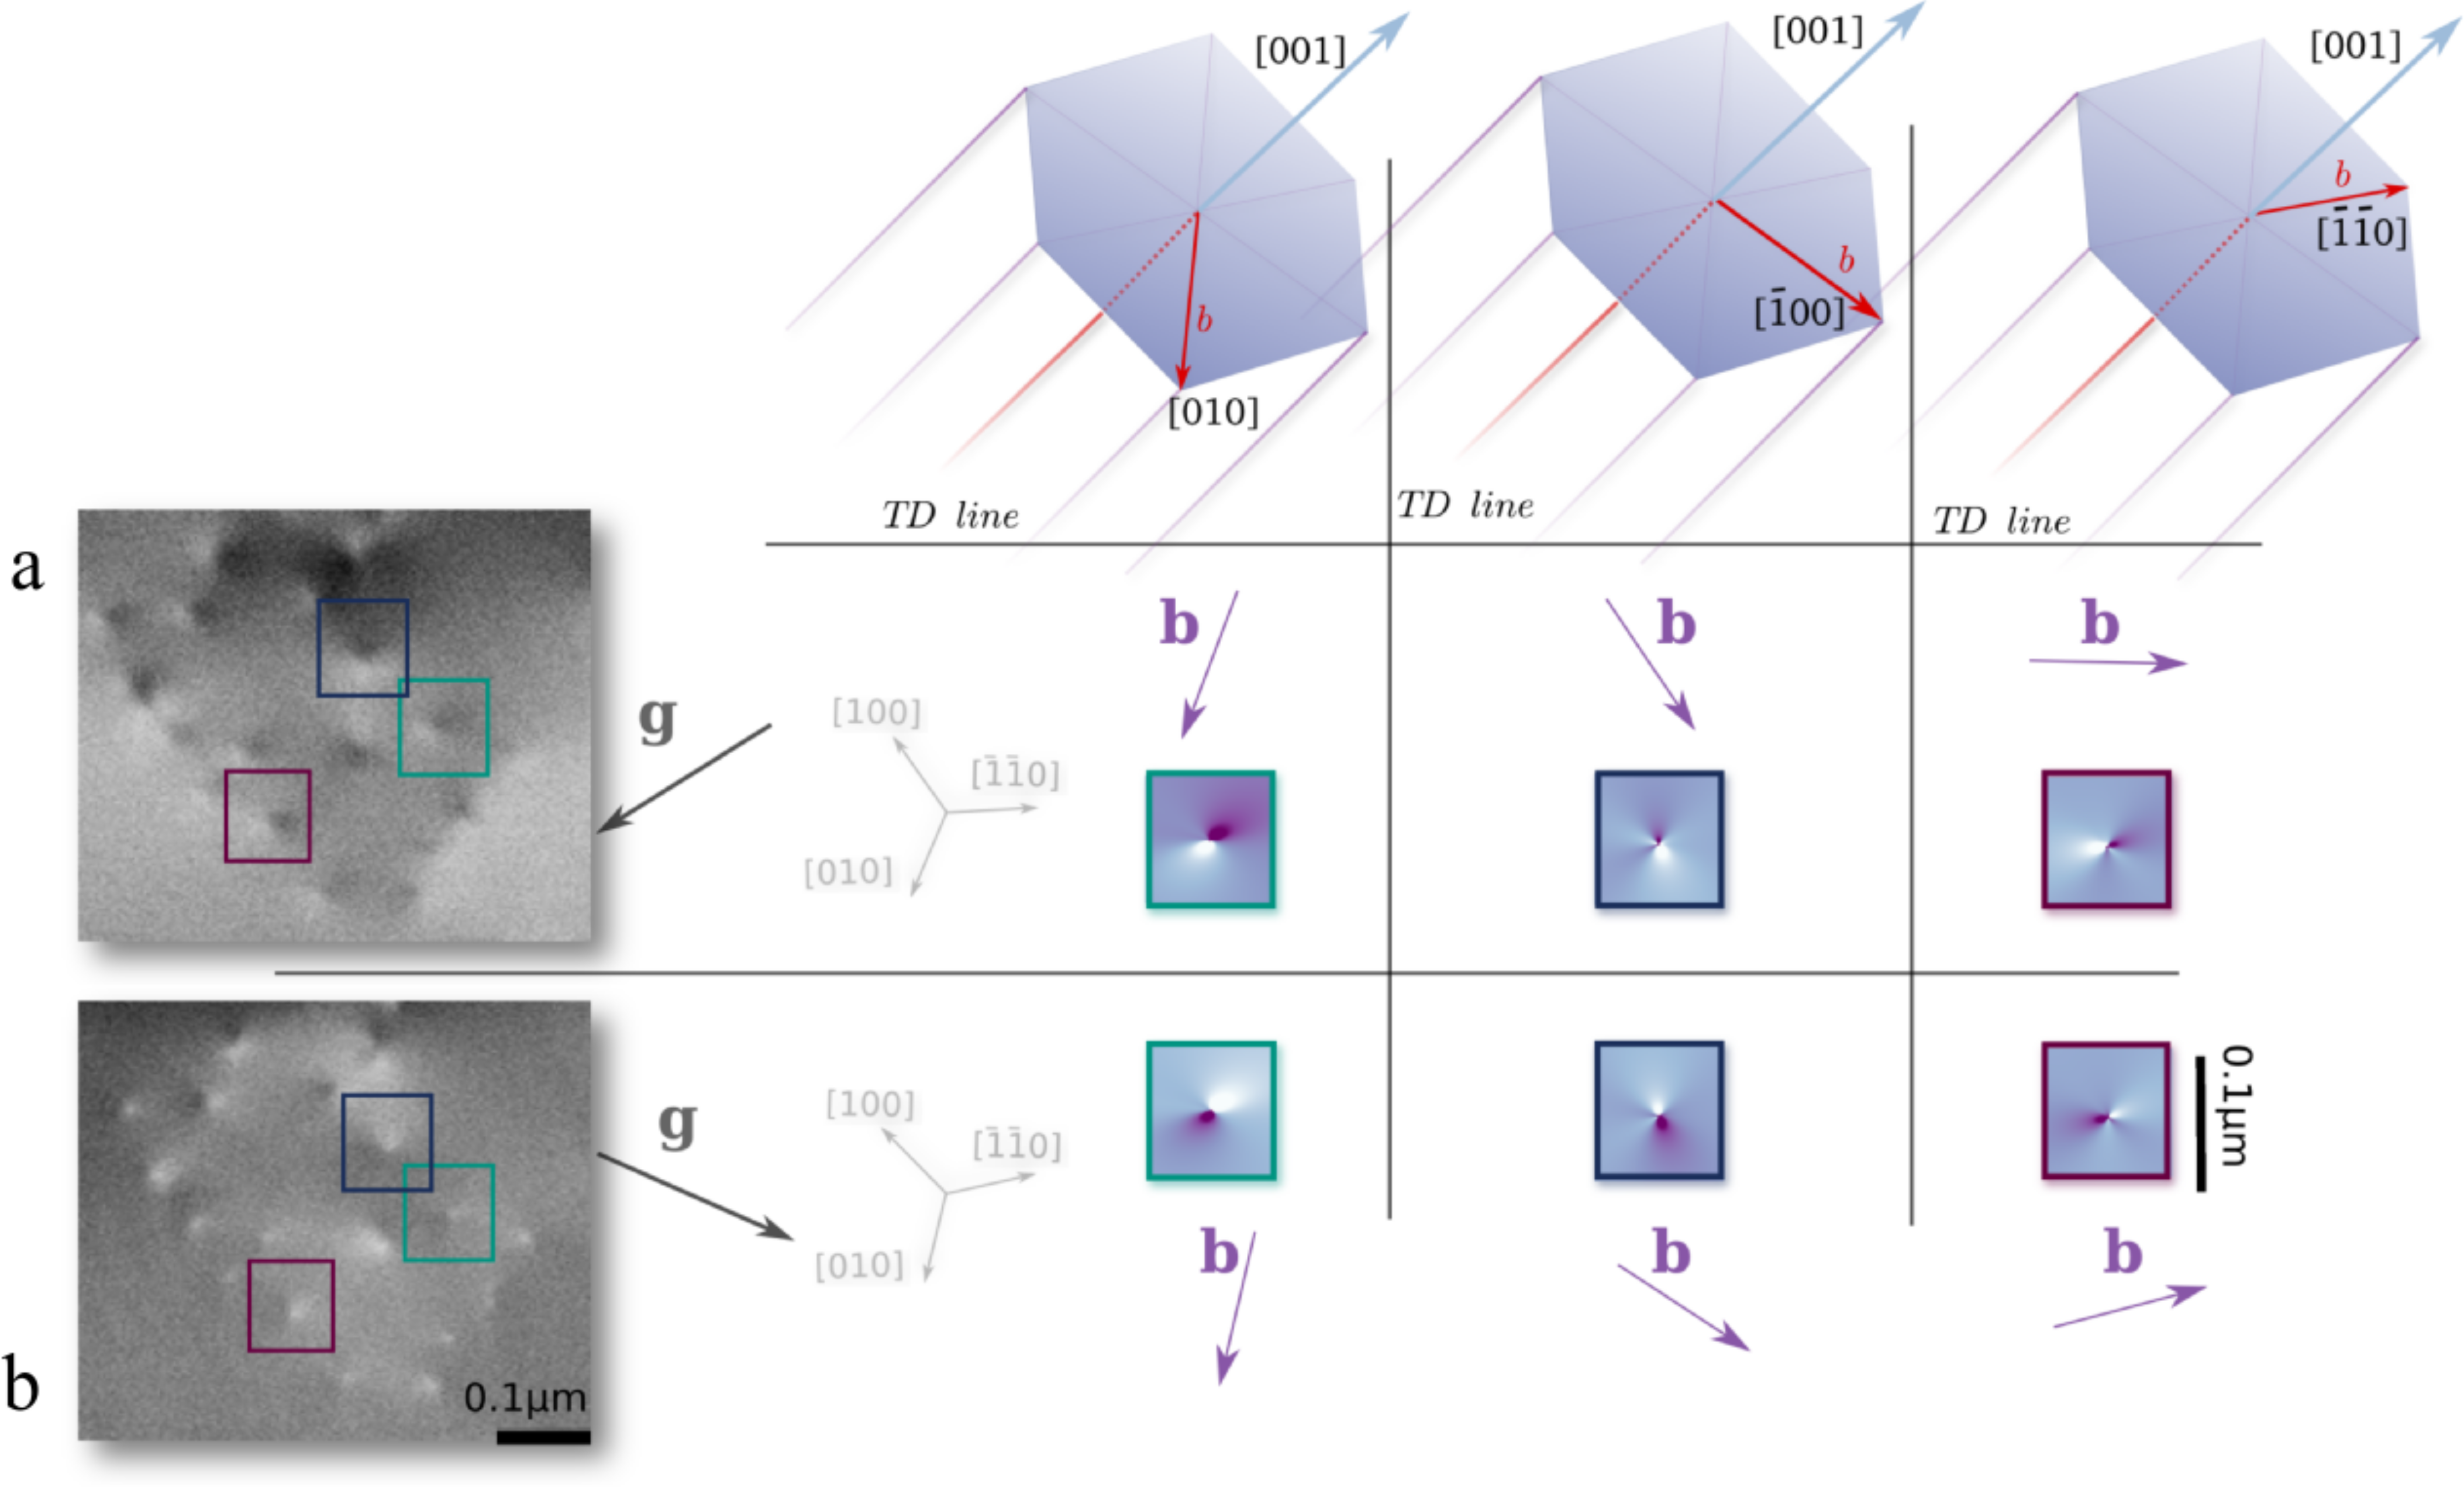
\includegraphics[width=1\linewidth]{Figures/contrast.png}
    \caption[Predicted contrast comparison with experiments.]{ Experimental images on the left (see page \ref{Naresh} for details) versus predicted edge TD dark-bright contrast in ECC images on the right. The two experimental images a) and b) are from the same area but the crystal has been tilted a few degrees to access the new diffraction condition. The boxes correspond to the contrast produced by an edge TD with \textbf{b} = [010] (green box),\textbf{ b} = [-100] (dark blue box), \textbf{b} = [-1-10] (purple box). See details in text. The Bravais three index notation was used throughout.}
    \label{fig:contrast}
\end{figure}

\begin{table}[ht]
    \centering
    \begin{tabular}{l l c}
    \toprule
        \tabhead{Parameter}     & \tabhead{Symbol} & \tabhead{Value}  \\
    \midrule    
         Extinction distance    & $\xi_g$         & \SI{29.6}{\nano \meter}  \\
         Beam penetration depth & $r^{max}_{inc}$ &  \SI{80}{\nano \meter}\\
    \bottomrule     
    \end{tabular}
    \caption[Modelling parameters.]{Modelling parameters for edge TDs in wurtzite GaN for the channelling conditions given in the text.}
    \label{Table:params}
\end{table}

The predicted contrasts shown are plotted as variation from the perfect crystal BSE yield. Namely, the calculated BSE intensity is normalised with respect to the BSE yield far away from the dislocation. Normalisation is not used when comparing with the experimental contrast images. The intensity is plotted using the BuPu multi-hue colour scheme with white showing the highest intensity, blue - intermediate values, and dark purple the lowest intensity.

A very similar behaviour to the strain field profile in a plane is observed: the darker-lighter intensity appears to follow the Burgers vector direction. This points towards the fact that a qualitative prediction of TD behaviour can be achieved from a bare strain model correctly ``sampled''. In order to reduce the characterisation uncertainty a larger number of different diffraction conditions should be acquired.


\subsection{Equivalence between contrast and ECC-strain}

In the end, the only change in the crystal is the dislocation displacement field, which will  locally affect the phase of an incident electron beam. The $\beta$ correction term is what tells the dynamical equations to locally change the position of the reciprocal lattice point closer to the Ewald sphere, resulting in an increase in intensity, or further from it, resulting in a decrease in intensity. This is what we see in the SEM microrgraph as TD contrast. 

\begin{figure}[ht]
    \centering
    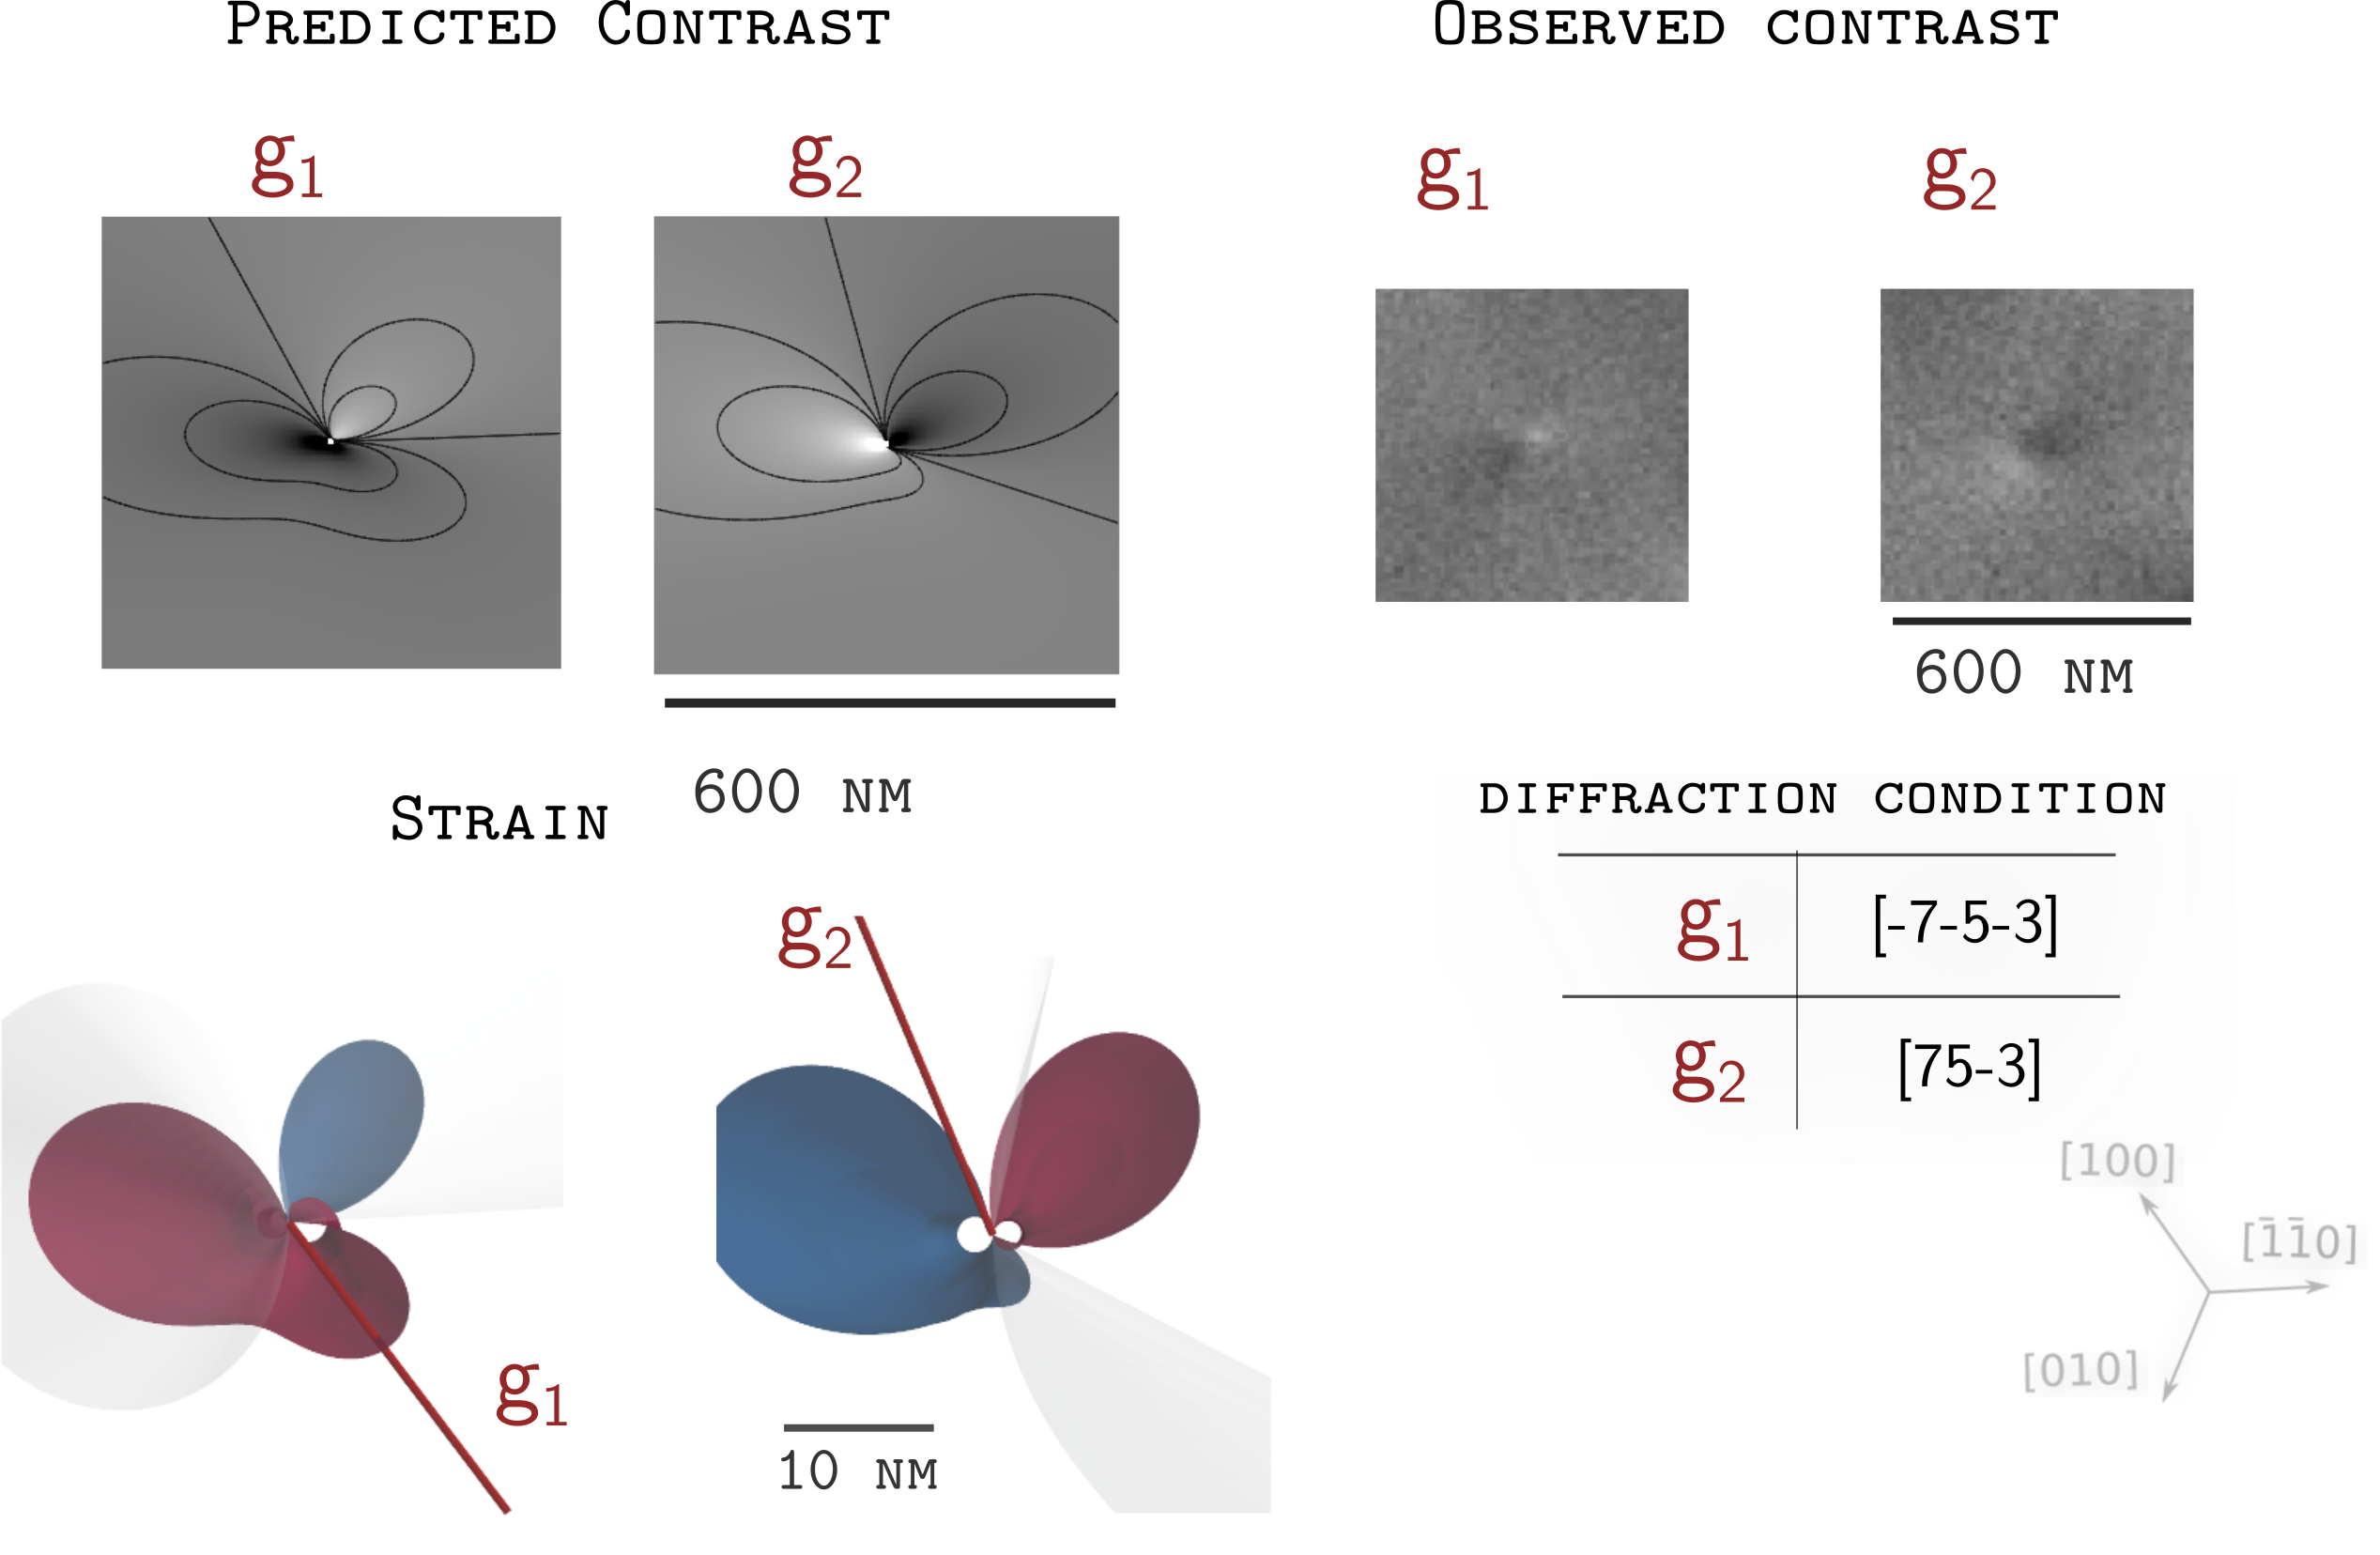
\includegraphics[width=0.7\linewidth]{Figures/screwcompare.png}
    \caption[ECC-strain vs contrast for a screw TD]{  Comparison between ECC-strain (bottom left) and contrast (top left) for a screw TD in two different diffraction conditions $\textbf{g}_1$ and $\textbf{g}_2$ (given on the bottom right). On the top right two TDs from ECC images taken in the same conditions as the simulations are shown.}
    \label{fig:screwcompare}
\end{figure}


In the left columns of Fig.~\ref{fig:screwcompare} and Fig.~\ref{fig:edgecompare} I want to show that if I plot the ECC-strain isosurfaces and compare them to the two-beam dynamical simulation prediction of TD contrast they show the exact same geometry of features.  Again, I compare the contrast prediction to selected TDs in ECC images taken in the same diffraction conditions as the simulations shown in the right column.  The ECCIs were taken by Naresh-Kumar and can be found in this paper~\cite{Naresh}.

\begin{figure}[htb]
    \centering
    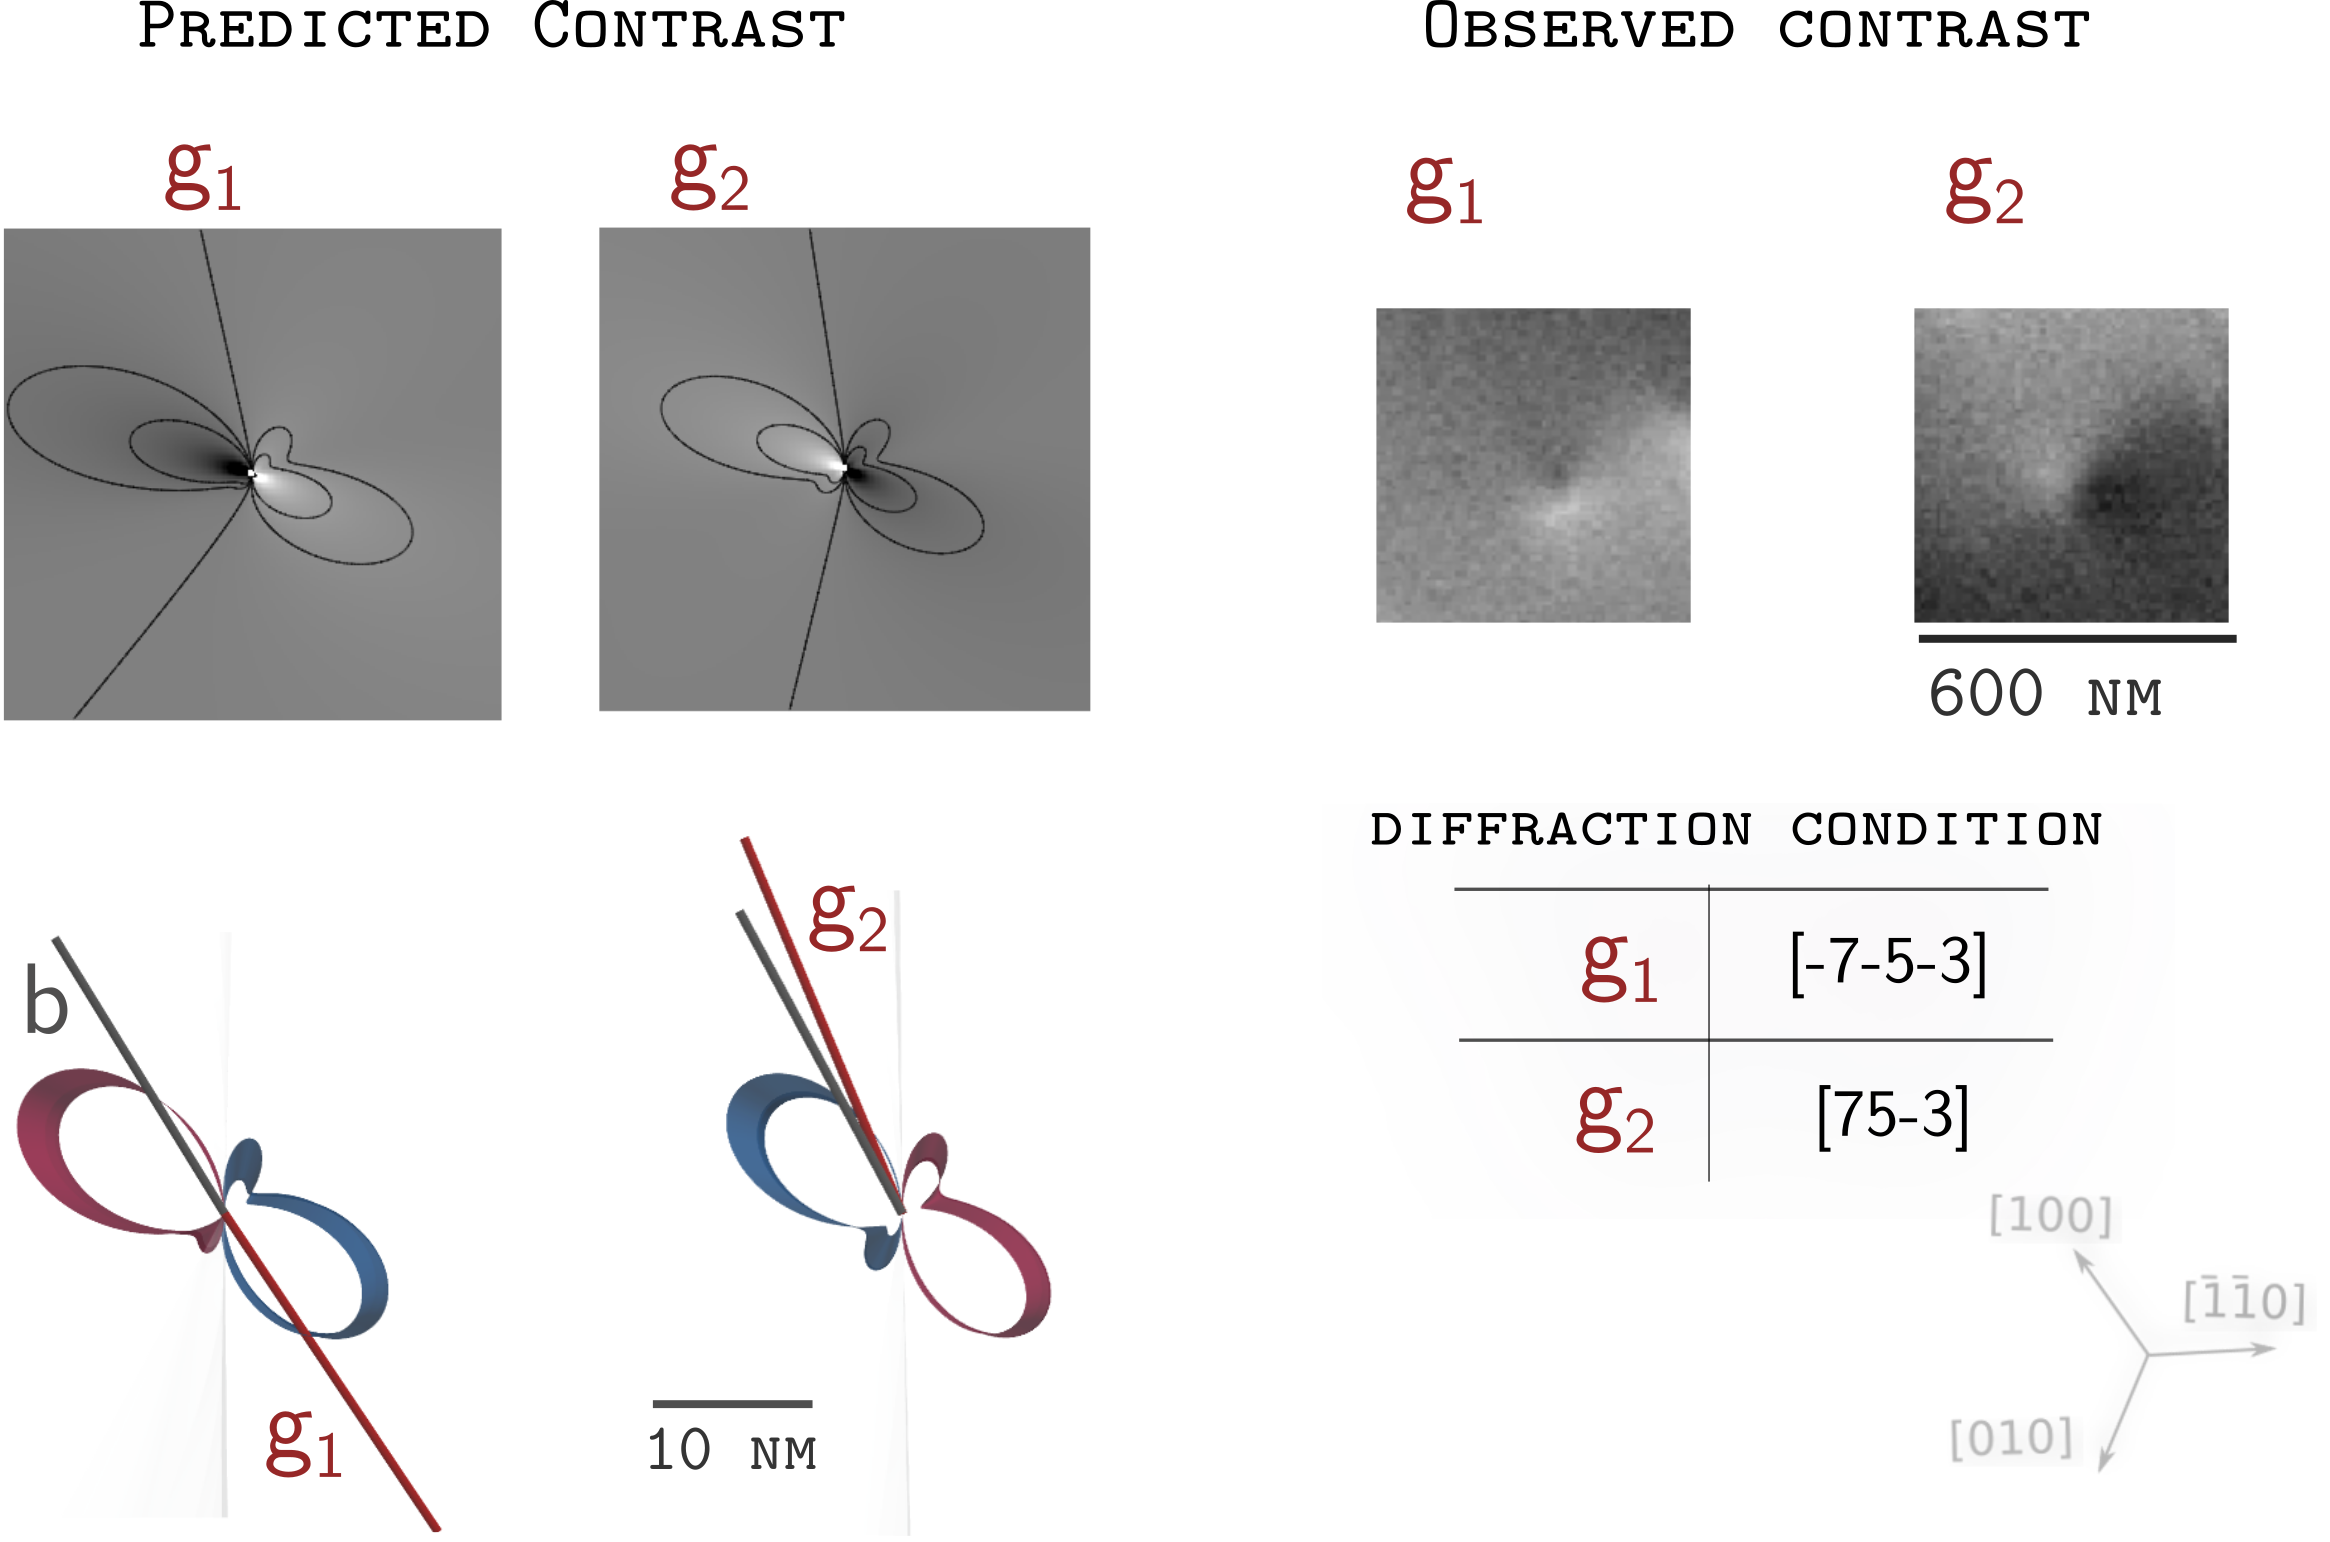
\includegraphics[width=0.7\linewidth]{Figures/edgecompare.png}
    \caption[ECC-strain vs contrast for an edge TD]{ Comparison between ECC-strain (bottom left) and contrast (top left) for an edge TD in two different diffraction conditions $\textbf{g}_1$ and $\textbf{g}_2$ (given on the bottom right). On top right two TDs from ECC images taken in the same conditions as the simulations are shown.}
    \label{fig:edgecompare}

 \vspace*{\floatsep}

    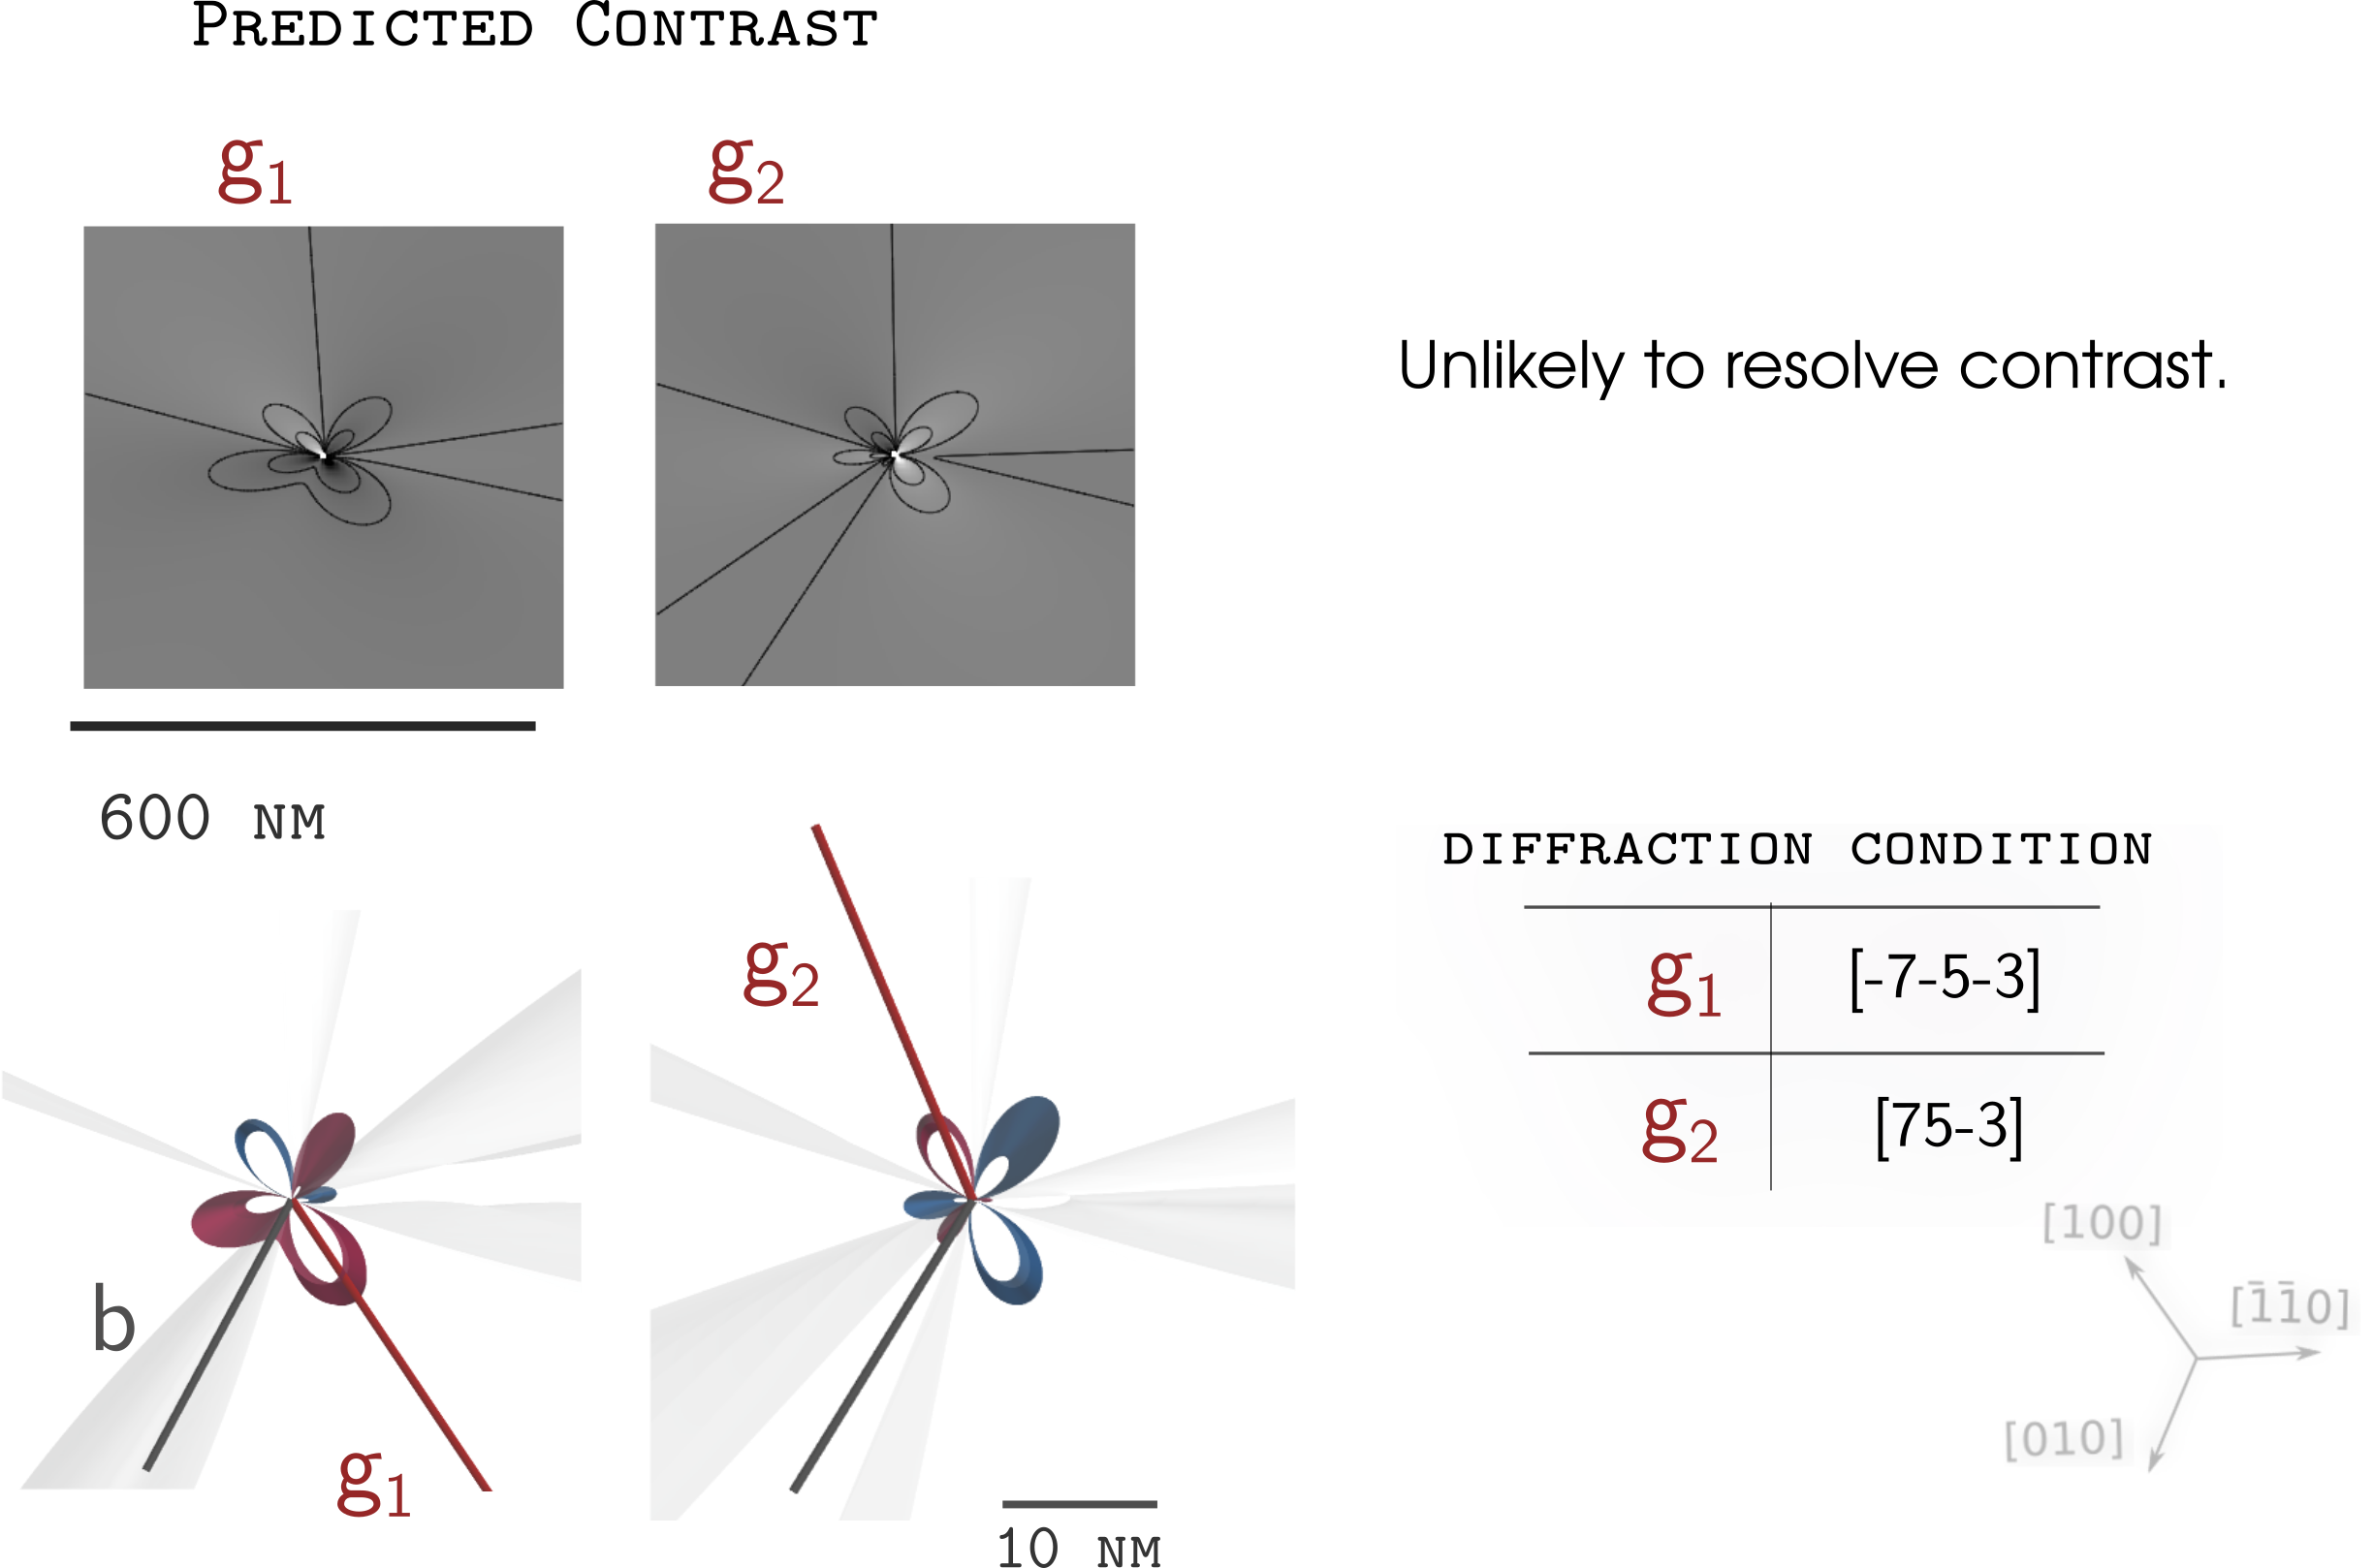
\includegraphics[width=0.7\linewidth]{Figures/edgecompare0.png}
    \caption[Vanishing ECC-strain vs vanishing contrast for an edge TD]{ Comparison between vanishing ECC-strain (bottom left) and vanishing contrast (top left) for an edge TD in two different diffraction conditions $\textbf{g}_1$ and $\textbf{g}_2$ (given on the bottom right).}
    \label{fig:edgecompare0}
\end{figure}


Fig.~\ref{fig:screwcompare} shows the top surface view strain isosurfaces (bottom) of a screw TD in two different diffraction conditions $\mathbf{g_1}$ and $\mathbf{g_2}$, whose projections on the viewing plane is shown as red rods. Like before the modelled material is \hkl[001] GaN and red strain isosurface indicated compressive strain (positive) while blue isosurface indicates tensile strain (negative). As discussed on page~\pageref{fig:edge}, for a screw TD in forward-scattering geometry the ECC-strain will be significant close to the surface. 

The calculated dynamical contrast (top figures) follows very closely the surface relaxation isosurface profile, with high intensity mapping the tensile strain introduced by the dislocation, and low intensity matching the compressive part. This matching behaviour is not straightforward to generalise. Looking back at the rocking curves on page~\pageref{Fig:rocking}, Fig.~\ref{Fig:rocking}, and remembering that the contrast in the SEM has contributions from both the incident and diffracted beam, we can see that small variations in intensity occur with deviation from Bragg  condition in a complex manner. Additionally, the rocking curves will look different for different diffraction conditions and integration depths. My argument here is that the ``proportionality factor'' between ECC-strain and intensity is non-trivial and simulations are required in order to predict the correct contrast. 



A very similar behaviour is observed for an edge TD and is shown in Fig.~\ref{fig:edgecompare}. This time the surface relaxation is not as prominent and we mostly see the infinite dislocation strain components. Nevertheless the features of these strain components can be rediscovered in the contrast simulations. The TDs in the experimental images show the same contrast geometry, perhaps with higher intensity than my predictions. Note that my simple simulations do not take into account any texture on surface of the sample, or perhaps more problematic, low angle grains between which the dislocations are commonly found. I will discuss more about this in Chapter~\ref{chap:Conclusion} on page~\pageref{chap:Conclusion}.


I conclude from these comparisons that it is the ECC-strain that gives the features of the contrast profile we observe in the SEM. If we are interested in understanding what the ECCI TD contrast tells us about the dislocation observed then we ``simply'' need to simulate the ECC-strain. The simulation involves juggling a number of different frames as we have seen on page~\pageref{sec:coordinates} which, in turn, requires a good understanding not only of coordinates transformation calculations which we covered in the introductory chapter, but also of the diffraction condition and exact beam-sample-detector geometry. Unfortunately, none of these are obvious in an SEM since the SEM is not optimised for diffraction, especially not for channelling in the same way the TEM is. Everything from the small and controlled interaction volume designed for TEM to the detector position optimised to maximise diffraction signal in diffraction mode are incongruous with the SEM. 
 





We can also see that for certain dislocation geometries like the one in Fig.~\ref{fig:edgecompare0} where the strain isosurfaces come very close to the core of the dislocation, \ie reduced ECC-strain, the contrast predicted will become faint. We do expect, then, that some dislocation can appear faint in the ECC images. If we were interested in a good approximation of their density, we would have to acquire multiple images in different diffraction conditions. 

\clearpage



\section{Conclusions}
ECCI can be used as an alternative to, or jointly with, the established defect characterisation techniques. Since the usual defect identification procedure developed for TEM is not entirely appropriate for looking at TDs in ECCI, modelling the contrast predictions becomes critical. 

The forescatter ECC images provide TD contrast features as cumulative sampled strain components defined in the Cartesian frames selected by the imaging diffraction condition. While the characterisation is more involved than in TEM, which benefits from the applicability of the 'invisibility criteria', simulations of ECCI dislocation strain profile can predict the observed dislocation contrast. As these features are unique for different dislocation characters, this technique can be used to identify the type of imaged dislocations by comparison between measured and simulated TDs. We propose that the ECCI dislocation contrast is uniquely predicted by the ECCI strain profile. The equivalence between ECCI strain and ECCI contrast can aid not only the physical understanding of the observed images but can predict the behaviour of the contrast. For instance, we can predict that the contrast profile will always follow the edge component of the Burgers vector and that the diffraction condition will not affect its symmetry.


Finally, I show qualitative agreement between predictions of TD contrast in ECC images for two different diffraction conditions and the experimental images. These types of calculations can be used to  unambiguously identify  the type of dislocation observed in ECCIs. 


If you can, reader, take an ECP before trying to find dislocation contrast in the SEM, even if it is poor quality you can use it to navigate towards a band, close to a Bragg condition and increase your chances of success. 



      
